\documentclass[twoside]{book}

% Packages required by doxygen
\usepackage{fixltx2e}
\usepackage{calc}
\usepackage{doxygen}
\usepackage[export]{adjustbox} % also loads graphicx
\usepackage{graphicx}
\usepackage[utf8]{inputenc}
\usepackage{makeidx}
\usepackage{multicol}
\usepackage{multirow}
\PassOptionsToPackage{warn}{textcomp}
\usepackage{textcomp}
\usepackage[nointegrals]{wasysym}
\usepackage[table]{xcolor}

% Font selection
\usepackage[T1]{fontenc}
\usepackage[scaled=.90]{helvet}
\usepackage{courier}
\usepackage{amssymb}
\usepackage{sectsty}
\renewcommand{\familydefault}{\sfdefault}
\allsectionsfont{%
  \fontseries{bc}\selectfont%
  \color{darkgray}%
}
\renewcommand{\DoxyLabelFont}{%
  \fontseries{bc}\selectfont%
  \color{darkgray}%
}
\newcommand{\+}{\discretionary{\mbox{\scriptsize$\hookleftarrow$}}{}{}}

% Page & text layout
\usepackage{geometry}
\geometry{%
  a4paper,%
  top=2.5cm,%
  bottom=2.5cm,%
  left=2.5cm,%
  right=2.5cm%
}
\tolerance=750
\hfuzz=15pt
\hbadness=750
\setlength{\emergencystretch}{15pt}
\setlength{\parindent}{0cm}
\setlength{\parskip}{3ex plus 2ex minus 2ex}
\makeatletter
\renewcommand{\paragraph}{%
  \@startsection{paragraph}{4}{0ex}{-1.0ex}{1.0ex}{%
    \normalfont\normalsize\bfseries\SS@parafont%
  }%
}
\renewcommand{\subparagraph}{%
  \@startsection{subparagraph}{5}{0ex}{-1.0ex}{1.0ex}{%
    \normalfont\normalsize\bfseries\SS@subparafont%
  }%
}
\makeatother

% Headers & footers
\usepackage{fancyhdr}
\pagestyle{fancyplain}
\fancyhead[LE]{\fancyplain{}{\bfseries\thepage}}
\fancyhead[CE]{\fancyplain{}{}}
\fancyhead[RE]{\fancyplain{}{\bfseries\leftmark}}
\fancyhead[LO]{\fancyplain{}{\bfseries\rightmark}}
\fancyhead[CO]{\fancyplain{}{}}
\fancyhead[RO]{\fancyplain{}{\bfseries\thepage}}
\fancyfoot[LE]{\fancyplain{}{}}
\fancyfoot[CE]{\fancyplain{}{}}
\fancyfoot[RE]{\fancyplain{}{\bfseries\scriptsize Generated by Doxygen }}
\fancyfoot[LO]{\fancyplain{}{\bfseries\scriptsize Generated by Doxygen }}
\fancyfoot[CO]{\fancyplain{}{}}
\fancyfoot[RO]{\fancyplain{}{}}
\renewcommand{\footrulewidth}{0.4pt}
\renewcommand{\chaptermark}[1]{%
  \markboth{#1}{}%
}
\renewcommand{\sectionmark}[1]{%
  \markright{\thesection\ #1}%
}

% Indices & bibliography
\usepackage{natbib}
\usepackage[titles]{tocloft}
\setcounter{tocdepth}{3}
\setcounter{secnumdepth}{5}
\makeindex

% Hyperlinks (required, but should be loaded last)
\usepackage{ifpdf}
\ifpdf
  \usepackage[pdftex,pagebackref=true]{hyperref}
\else
  \usepackage[ps2pdf,pagebackref=true]{hyperref}
\fi
\hypersetup{%
  colorlinks=true,%
  linkcolor=blue,%
  citecolor=blue,%
  unicode%
}

% Custom commands
\newcommand{\clearemptydoublepage}{%
  \newpage{\pagestyle{empty}\cleardoublepage}%
}

\usepackage{caption}
\captionsetup{labelsep=space,justification=centering,font={bf},singlelinecheck=off,skip=4pt,position=top}

%===== C O N T E N T S =====

\begin{document}

% Titlepage & ToC
\hypersetup{pageanchor=false,
             bookmarksnumbered=true,
             pdfencoding=unicode
            }
\pagenumbering{alph}
\begin{titlepage}
\vspace*{7cm}
\begin{center}%
{\Large M\+O\+H\+I\+D\+Lagrangian \\[1ex]\large 0.\+01 }\\
\vspace*{1cm}
{\large Generated by Doxygen 1.8.14}\\
\end{center}
\end{titlepage}
\clearemptydoublepage
\pagenumbering{roman}
\tableofcontents
\clearemptydoublepage
\pagenumbering{arabic}
\hypersetup{pageanchor=true}

%--- Begin generated contents ---
\chapter{Modules Index}
\section{Modules List}
Here is a list of all modules with brief descriptions\+:\begin{DoxyCompactList}
\item\contentsline{section}{\mbox{\hyperlink{namespaceabstract__linkedlist__mod}{abstract\+\_\+linkedlist\+\_\+mod}} \\*Module that defines an unlimited polymorphic container list class and related methods. A container is a fundamental entity allowing to build data structures such as lists and arrays. This is an abstract type, so a derived type must be defined for any specific contents that may be required. Those derived types should provide type-\/specific methods that require type-\/guards, such as printing }{\pageref{namespaceabstract__linkedlist__mod}}{}
\item\contentsline{section}{\mbox{\hyperlink{namespaceaot__mod}{aot\+\_\+mod}} \\*Module to hold the Arrays of Tracers class and its methods. This class defines a collection of id, xyz, uvw, .. arrays that allow for easy and efficient manipulation of the Tracer objects. These must be exported into the objects from this class }{\pageref{namespaceaot__mod}}{}
\item\contentsline{section}{\mbox{\hyperlink{namespacebackground__mod}{background\+\_\+mod}} \\*Defines a background class that describes a solution from which to interpolate. A background object contains an arbitrary number of scalar or vectorial fields, in 2, 3 or 4D, indexed to labeled 1D fields of dimensions. The fields are stored in a linked list, enabling trivial iteration }{\pageref{namespacebackground__mod}}{}
\item\contentsline{section}{\mbox{\hyperlink{namespaceblocks__mod}{blocks\+\_\+mod}} \\*Module that defines a block class and related methods. A block is a fundamental type of the model. It contains a sub-\/domain of the simulation bounding box, holding all entities inside that sub-\/domain. It maps to a domain decomposition parallelization strategy, if needed }{\pageref{namespaceblocks__mod}}{}
\item\contentsline{section}{\mbox{\hyperlink{namespaceboundingbox__mod}{boundingbox\+\_\+mod}} \\*Module that defines a simulation Bounding Box }{\pageref{namespaceboundingbox__mod}}{}
\item\contentsline{section}{\mbox{\hyperlink{namespacecommon__modules}{common\+\_\+modules}} \\*Module to hold all of the commonly used base modules }{\pageref{namespacecommon__modules}}{}
\item\contentsline{section}{\mbox{\hyperlink{namespacecontainer__mod}{container\+\_\+mod}} \\*Module that defines an unlimited polymorphic container class and related methods. A container is a fundamental entity allowing to build data structures such as lists and arrays }{\pageref{namespacecontainer__mod}}{}
\item\contentsline{section}{\mbox{\hyperlink{namespaceemitter__mod}{emitter\+\_\+mod}} \\*Module that defines an emitter class and related methods. This module is responsible for building a potential tracer list based on the availble sources and calling their initializers }{\pageref{namespaceemitter__mod}}{}
\item\contentsline{section}{\mbox{\hyperlink{namespacefield__types__mod}{field\+\_\+types\+\_\+mod}} \\*Defines classes for \textquotesingle{}fields\textquotesingle{}\+: 1, 2, 3 and 4D labeled data. Valid for both scalar and vectorial (real) data. Defines a generic wrapper for these classes, that abstracts the user from having to choose their data dimensionality or type to create a field }{\pageref{namespacefield__types__mod}}{}
\item\contentsline{section}{\mbox{\hyperlink{namespacegeometry__mod}{geometry\+\_\+mod}} \\*Module that defines geometry classes and related methods }{\pageref{namespacegeometry__mod}}{}
\item\contentsline{section}{\mbox{\hyperlink{namespaceinterpolator__mod}{interpolator\+\_\+mod}} \\*Defines an Interpolator class }{\pageref{namespaceinterpolator__mod}}{}
\item\contentsline{section}{\mbox{\hyperlink{namespacelink__mod}{link\+\_\+mod}} \\*Module that defines a link based on an unlimited polymorphic container class }{\pageref{namespacelink__mod}}{}
\item\contentsline{section}{\mbox{\hyperlink{namespacesimulation__about__mod}{simulation\+\_\+about\+\_\+mod}} \\*Module to print version, licence, preambles }{\pageref{namespacesimulation__about__mod}}{}
\item\contentsline{section}{\mbox{\hyperlink{namespacesimulation__globals__mod}{simulation\+\_\+globals\+\_\+mod}} \\*Module to hold the simulation global parameter classes and their methods }{\pageref{namespacesimulation__globals__mod}}{}
\item\contentsline{section}{\mbox{\hyperlink{namespacesimulation__initialize__mod}{simulation\+\_\+initialize\+\_\+mod}} \\*Module with the simulation initialization related definitions and methods. Has one public access routine that is incharge of building the simulation space from input files }{\pageref{namespacesimulation__initialize__mod}}{}
\item\contentsline{section}{\mbox{\hyperlink{namespacesimulation__logger__mod}{simulation\+\_\+logger\+\_\+mod}} \\*Module to hold all the simulation logger related definitions and methods }{\pageref{namespacesimulation__logger__mod}}{}
\item\contentsline{section}{\mbox{\hyperlink{namespacesimulation__memory__mod}{simulation\+\_\+memory\+\_\+mod}} \\*Module to hold the simulation memory managment class and its methods }{\pageref{namespacesimulation__memory__mod}}{}
\item\contentsline{section}{\mbox{\hyperlink{namespacesimulation__mod}{simulation\+\_\+mod}} \\*Module to hold the simulation class and its methods. This is the only class that is exposed to an external program, as it encapsulates every other class and method }{\pageref{namespacesimulation__mod}}{}
\item\contentsline{section}{\mbox{\hyperlink{namespacesimulation__output__streamer__mod}{simulation\+\_\+output\+\_\+streamer\+\_\+mod}} \\*Defines a output file writer class with an object exposable to the Simulation This class is in charge of selectig the correct writter for the selected output file format }{\pageref{namespacesimulation__output__streamer__mod}}{}
\item\contentsline{section}{\mbox{\hyperlink{namespacesimulation__precision__mod}{simulation\+\_\+precision\+\_\+mod}} \\*Module to control the precision of the variables trough the project }{\pageref{namespacesimulation__precision__mod}}{}
\item\contentsline{section}{\mbox{\hyperlink{namespacesolver__mod}{solver\+\_\+mod}} \\*Defines an Solver class. This class invokes the different available integration algorithms as methods, and these invoke the necessary interpolation objects }{\pageref{namespacesolver__mod}}{}
\item\contentsline{section}{\mbox{\hyperlink{namespacesources__list__mod}{sources\+\_\+list\+\_\+mod}} \\*Module to hold the Sources linked list class and its methods. This class defines a double linked list to store any variable type, but with specific methods with type guards for Source objects. The class allows for insertion, deletion and iteration of the desired contents }{\pageref{namespacesources__list__mod}}{}
\item\contentsline{section}{\mbox{\hyperlink{namespacesources__mod}{sources\+\_\+mod}} \\*Module that defines a source class and related methods }{\pageref{namespacesources__mod}}{}
\item\contentsline{section}{\mbox{\hyperlink{namespacetracer__base__mod}{tracer\+\_\+base\+\_\+mod}} \\*Module that defines a pure Lagrangian tracer class and related methods }{\pageref{namespacetracer__base__mod}}{}
\item\contentsline{section}{\mbox{\hyperlink{namespacetracer__list__mod}{tracer\+\_\+list\+\_\+mod}} \\*Module to hold the tracer linked list class and its methods. This class defines a double linked list to store any variable type, but with specific methods with type guards for Tracer objects. The class allows for insertion, deletion and iteration of the desired contents }{\pageref{namespacetracer__list__mod}}{}
\item\contentsline{section}{\mbox{\hyperlink{namespacetracer__paper__mod}{tracer\+\_\+paper\+\_\+mod}} \\*Module that defines a Lagrangian tracer class for paper modelling and related methods. The type is defined as a derived type from the pule Lagrangian tracer, and hence inherits all of it\textquotesingle{}s data and methods }{\pageref{namespacetracer__paper__mod}}{}
\item\contentsline{section}{\mbox{\hyperlink{namespacetracer__plastic__mod}{tracer\+\_\+plastic\+\_\+mod}} \\*Module that defines a Lagrangian tracer class for plastic modelling and related methods. The type is defined as a derived type from the pule Lagrangian tracer, and hence inherits all of it\textquotesingle{}s data and methods }{\pageref{namespacetracer__plastic__mod}}{}
\item\contentsline{section}{\mbox{\hyperlink{namespacetracers__mod}{tracers\+\_\+mod}} \\*Module to hold and \textquotesingle{}wrap\textquotesingle{} all the tracer respective modules }{\pageref{namespacetracers__mod}}{}
\item\contentsline{section}{\mbox{\hyperlink{namespaceutilities__mod}{utilities\+\_\+mod}} \\*Module that provides useful back-\/end routines }{\pageref{namespaceutilities__mod}}{}
\item\contentsline{section}{\mbox{\hyperlink{namespacevtkwritter__mod}{vtkwritter\+\_\+mod}} \\*Defines a vtk writer class with an object exposable to the Output streamer. Writes files in .xml vtk, both in serial and parallel model. Uses an unstructured mesh format specifier to store any type of data, both meshes and Tracers. Supports scalar and vectorial data }{\pageref{namespacevtkwritter__mod}}{}
\item\contentsline{section}{\mbox{\hyperlink{namespacexmlparser__mod}{xmlparser\+\_\+mod}} \\*Module with the simulation xml parsing class and methods, Encapsulates the F\+O\+X\+\_\+dom library }{\pageref{namespacexmlparser__mod}}{}
\end{DoxyCompactList}

\chapter{File Index}
\section{File List}
Here is a list of all files with brief descriptions\+:\begin{DoxyCompactList}
\item\contentsline{section}{C\+:/\+Users/administrator/\+Documents/\+Git\+Hub/\+M\+O\+H\+I\+D-\/\+Lagrangian/src/app/\mbox{\hyperlink{_m_o_h_i_d_lagrangian_8f90}{M\+O\+H\+I\+D\+Lagrangian.\+f90}} }{\pageref{_m_o_h_i_d_lagrangian_8f90}}{}
\item\contentsline{section}{C\+:/\+Users/administrator/\+Documents/\+Git\+Hub/\+M\+O\+H\+I\+D-\/\+Lagrangian/src/lib/\mbox{\hyperlink{about_8f90}{about.\+f90}} }{\pageref{about_8f90}}{}
\item\contentsline{section}{C\+:/\+Users/administrator/\+Documents/\+Git\+Hub/\+M\+O\+H\+I\+D-\/\+Lagrangian/src/lib/\mbox{\hyperlink{abstract__container__array_8f90}{abstract\+\_\+container\+\_\+array.\+f90}} }{\pageref{abstract__container__array_8f90}}{}
\item\contentsline{section}{C\+:/\+Users/administrator/\+Documents/\+Git\+Hub/\+M\+O\+H\+I\+D-\/\+Lagrangian/src/lib/\mbox{\hyperlink{blocks_8f90}{blocks.\+f90}} }{\pageref{blocks_8f90}}{}
\item\contentsline{section}{C\+:/\+Users/administrator/\+Documents/\+Git\+Hub/\+M\+O\+H\+I\+D-\/\+Lagrangian/src/lib/\mbox{\hyperlink{boundingbox_8f90}{boundingbox.\+f90}} }{\pageref{boundingbox_8f90}}{}
\item\contentsline{section}{C\+:/\+Users/administrator/\+Documents/\+Git\+Hub/\+M\+O\+H\+I\+D-\/\+Lagrangian/src/lib/\mbox{\hyperlink{common__modules_8f90}{common\+\_\+modules.\+f90}} }{\pageref{common__modules_8f90}}{}
\item\contentsline{section}{C\+:/\+Users/administrator/\+Documents/\+Git\+Hub/\+M\+O\+H\+I\+D-\/\+Lagrangian/src/lib/\mbox{\hyperlink{container_8f90}{container.\+f90}} }{\pageref{container_8f90}}{}
\item\contentsline{section}{C\+:/\+Users/administrator/\+Documents/\+Git\+Hub/\+M\+O\+H\+I\+D-\/\+Lagrangian/src/lib/\mbox{\hyperlink{emitter_8f90}{emitter.\+f90}} }{\pageref{emitter_8f90}}{}
\item\contentsline{section}{C\+:/\+Users/administrator/\+Documents/\+Git\+Hub/\+M\+O\+H\+I\+D-\/\+Lagrangian/src/lib/\mbox{\hyperlink{geometry_8f90}{geometry.\+f90}} }{\pageref{geometry_8f90}}{}
\item\contentsline{section}{C\+:/\+Users/administrator/\+Documents/\+Git\+Hub/\+M\+O\+H\+I\+D-\/\+Lagrangian/src/lib/\mbox{\hyperlink{initialize_8f90}{initialize.\+f90}} }{\pageref{initialize_8f90}}{}
\item\contentsline{section}{C\+:/\+Users/administrator/\+Documents/\+Git\+Hub/\+M\+O\+H\+I\+D-\/\+Lagrangian/src/lib/\mbox{\hyperlink{simulation_8f90}{simulation.\+f90}} }{\pageref{simulation_8f90}}{}
\item\contentsline{section}{C\+:/\+Users/administrator/\+Documents/\+Git\+Hub/\+M\+O\+H\+I\+D-\/\+Lagrangian/src/lib/\mbox{\hyperlink{simulation__globals_8f90}{simulation\+\_\+globals.\+f90}} }{\pageref{simulation__globals_8f90}}{}
\item\contentsline{section}{C\+:/\+Users/administrator/\+Documents/\+Git\+Hub/\+M\+O\+H\+I\+D-\/\+Lagrangian/src/lib/\mbox{\hyperlink{simulation__logger_8f90}{simulation\+\_\+logger.\+f90}} }{\pageref{simulation__logger_8f90}}{}
\item\contentsline{section}{C\+:/\+Users/administrator/\+Documents/\+Git\+Hub/\+M\+O\+H\+I\+D-\/\+Lagrangian/src/lib/\mbox{\hyperlink{simulation__memory_8f90}{simulation\+\_\+memory.\+f90}} }{\pageref{simulation__memory_8f90}}{}
\item\contentsline{section}{C\+:/\+Users/administrator/\+Documents/\+Git\+Hub/\+M\+O\+H\+I\+D-\/\+Lagrangian/src/lib/\mbox{\hyperlink{simulation__precision_8f90}{simulation\+\_\+precision.\+f90}} }{\pageref{simulation__precision_8f90}}{}
\item\contentsline{section}{C\+:/\+Users/administrator/\+Documents/\+Git\+Hub/\+M\+O\+H\+I\+D-\/\+Lagrangian/src/lib/\mbox{\hyperlink{simulation__xmlparser_8f90}{simulation\+\_\+xmlparser.\+f90}} }{\pageref{simulation__xmlparser_8f90}}{}
\item\contentsline{section}{C\+:/\+Users/administrator/\+Documents/\+Git\+Hub/\+M\+O\+H\+I\+D-\/\+Lagrangian/src/lib/\mbox{\hyperlink{sources_8f90}{sources.\+f90}} }{\pageref{sources_8f90}}{}
\item\contentsline{section}{C\+:/\+Users/administrator/\+Documents/\+Git\+Hub/\+M\+O\+H\+I\+D-\/\+Lagrangian/src/lib/\mbox{\hyperlink{sources__array_8f90}{sources\+\_\+array.\+f90}} }{\pageref{sources__array_8f90}}{}
\item\contentsline{section}{C\+:/\+Users/administrator/\+Documents/\+Git\+Hub/\+M\+O\+H\+I\+D-\/\+Lagrangian/src/lib/\mbox{\hyperlink{tracer__array_8f90}{tracer\+\_\+array.\+f90}} }{\pageref{tracer__array_8f90}}{}
\item\contentsline{section}{C\+:/\+Users/administrator/\+Documents/\+Git\+Hub/\+M\+O\+H\+I\+D-\/\+Lagrangian/src/lib/\mbox{\hyperlink{tracer__base_8f90}{tracer\+\_\+base.\+f90}} }{\pageref{tracer__base_8f90}}{}
\item\contentsline{section}{C\+:/\+Users/administrator/\+Documents/\+Git\+Hub/\+M\+O\+H\+I\+D-\/\+Lagrangian/src/lib/\mbox{\hyperlink{tracer__interp_8f90}{tracer\+\_\+interp.\+f90}} }{\pageref{tracer__interp_8f90}}{}
\item\contentsline{section}{C\+:/\+Users/administrator/\+Documents/\+Git\+Hub/\+M\+O\+H\+I\+D-\/\+Lagrangian/src/lib/\mbox{\hyperlink{tracer__paper_8f90}{tracer\+\_\+paper.\+f90}} }{\pageref{tracer__paper_8f90}}{}
\item\contentsline{section}{C\+:/\+Users/administrator/\+Documents/\+Git\+Hub/\+M\+O\+H\+I\+D-\/\+Lagrangian/src/lib/\mbox{\hyperlink{tracer__plastic_8f90}{tracer\+\_\+plastic.\+f90}} }{\pageref{tracer__plastic_8f90}}{}
\item\contentsline{section}{C\+:/\+Users/administrator/\+Documents/\+Git\+Hub/\+M\+O\+H\+I\+D-\/\+Lagrangian/src/lib/\mbox{\hyperlink{tracers_8f90}{tracers.\+f90}} }{\pageref{tracers_8f90}}{}
\item\contentsline{section}{C\+:/\+Users/administrator/\+Documents/\+Git\+Hub/\+M\+O\+H\+I\+D-\/\+Lagrangian/src/lib/\mbox{\hyperlink{utilities_8f90}{utilities.\+f90}} }{\pageref{utilities_8f90}}{}
\end{DoxyCompactList}

\chapter{Module Documentation}
\hypertarget{namespacecommom__modules}{}\section{commom\+\_\+modules Module Reference}
\label{namespacecommom__modules}\index{commom\+\_\+modules@{commom\+\_\+modules}}


Module to hold all of the commonly used base modules.  




\subsection{Detailed Description}
Module to hold all of the commonly used base modules. 

\begin{DoxyAuthor}{Author}
Ricardo Birjukovs Canelas 
\end{DoxyAuthor}

\hypertarget{namespaceinitialize}{}\section{initialize Module Reference}
\label{namespaceinitialize}\index{initialize@{initialize}}


Module with the simulation initialization related definitions and methods. Has one public access routine that is incharge of building the simulation space from input files.  


\subsection*{Functions/\+Subroutines}
\begin{DoxyCompactItemize}
\item 
subroutine \mbox{\hyperlink{namespaceinitialize_ab91b27efd537a161ee9ca4b2d9efde1a}{linkpropertysources}} (links\+Node)
\begin{DoxyCompactList}\small\item\em Birjukovs Canelas -\/ M\+A\+R\+E\+T\+EC \end{DoxyCompactList}\item 
subroutine \mbox{\hyperlink{namespaceinitialize_a4640ad15e29b88467ec842f274f64b62}{init\+\_\+properties}} (case\+\_\+node)
\begin{DoxyCompactList}\small\item\em Birjukovs Canelas -\/ M\+A\+R\+E\+T\+EC \end{DoxyCompactList}\item 
subroutine \mbox{\hyperlink{namespaceinitialize_ad36e4f602dab66c06a1f0e2474e9f0a6}{read\+\_\+xml\+\_\+geometry}} (source, source\+\_\+detail, geometry)
\begin{DoxyCompactList}\small\item\em Birjukovs Canelas -\/ M\+A\+R\+E\+T\+EC \end{DoxyCompactList}\item 
subroutine \mbox{\hyperlink{namespaceinitialize_a9ed75476e5dd07928aed3442281930be}{init\+\_\+sources}} (case\+\_\+node)
\begin{DoxyCompactList}\small\item\em Birjukovs Canelas -\/ M\+A\+R\+E\+T\+EC \end{DoxyCompactList}\item 
subroutine \mbox{\hyperlink{namespaceinitialize_adb972e92da4789506ee6b62b702df2b3}{init\+\_\+simdefs}} (case\+\_\+node)
\begin{DoxyCompactList}\small\item\em Birjukovs Canelas -\/ M\+A\+R\+E\+T\+EC \end{DoxyCompactList}\item 
subroutine \mbox{\hyperlink{namespaceinitialize_a4c982b312ab10bf112dd3d2bc314569e}{init\+\_\+caseconstants}} (case\+\_\+node)
\begin{DoxyCompactList}\small\item\em Birjukovs Canelas -\/ M\+A\+R\+E\+T\+EC \end{DoxyCompactList}\item 
subroutine \mbox{\hyperlink{namespaceinitialize_a7a54dc126f448bea2b566339a449f85c}{init\+\_\+parameters}} (execution\+\_\+node)
\begin{DoxyCompactList}\small\item\em Birjukovs Canelas -\/ M\+A\+R\+E\+T\+EC \end{DoxyCompactList}\item 
subroutine, public \mbox{\hyperlink{namespaceinitialize_a45b7ca20c45cf272acbc391950cbb804}{initmohidlagrangian}} (xmlfilename)
\begin{DoxyCompactList}\small\item\em Birjukovs Canelas -\/ M\+A\+R\+E\+T\+EC \end{DoxyCompactList}\end{DoxyCompactItemize}


\subsection{Detailed Description}
Module with the simulation initialization related definitions and methods. Has one public access routine that is incharge of building the simulation space from input files. 

\begin{DoxyAuthor}{Author}
Ricardo Birjukovs Canelas 
\end{DoxyAuthor}


\subsection{Function/\+Subroutine Documentation}
\mbox{\Hypertarget{namespaceinitialize_a4c982b312ab10bf112dd3d2bc314569e}\label{namespaceinitialize_a4c982b312ab10bf112dd3d2bc314569e}} 
\index{initialize@{initialize}!init\+\_\+caseconstants@{init\+\_\+caseconstants}}
\index{init\+\_\+caseconstants@{init\+\_\+caseconstants}!initialize@{initialize}}
\subsubsection{\texorpdfstring{init\+\_\+caseconstants()}{init\_caseconstants()}}
{\footnotesize\ttfamily subroutine initialize\+::init\+\_\+caseconstants (\begin{DoxyParamCaption}\item[{type(node), intent(in), pointer}]{case\+\_\+node }\end{DoxyParamCaption})\hspace{0.3cm}{\ttfamily [private]}}



Birjukovs Canelas -\/ M\+A\+R\+E\+T\+EC 

Private case constant parser routine. Builds the simulation parametric space from the input xml case file. 
\begin{DoxyParams}[1]{Parameters}
\mbox{\tt in}  & {\em parsedxml} & \\
\hline
\end{DoxyParams}
Here is the call graph for this function\+:
\nopagebreak
\begin{figure}[H]
\begin{center}
\leavevmode
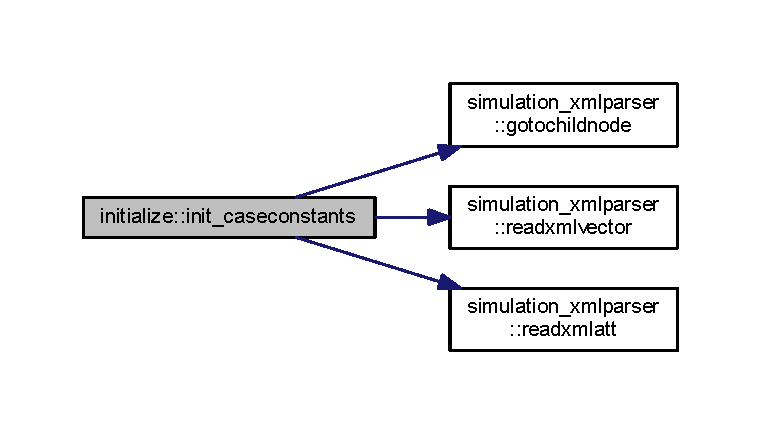
\includegraphics[width=350pt]{namespaceinitialize_a4c982b312ab10bf112dd3d2bc314569e_cgraph}
\end{center}
\end{figure}
Here is the caller graph for this function\+:
\nopagebreak
\begin{figure}[H]
\begin{center}
\leavevmode
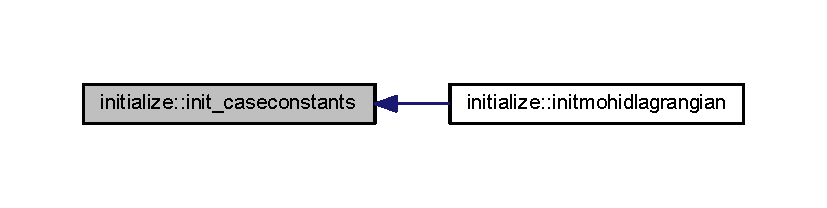
\includegraphics[width=350pt]{namespaceinitialize_a4c982b312ab10bf112dd3d2bc314569e_icgraph}
\end{center}
\end{figure}
\mbox{\Hypertarget{namespaceinitialize_a7a54dc126f448bea2b566339a449f85c}\label{namespaceinitialize_a7a54dc126f448bea2b566339a449f85c}} 
\index{initialize@{initialize}!init\+\_\+parameters@{init\+\_\+parameters}}
\index{init\+\_\+parameters@{init\+\_\+parameters}!initialize@{initialize}}
\subsubsection{\texorpdfstring{init\+\_\+parameters()}{init\_parameters()}}
{\footnotesize\ttfamily subroutine initialize\+::init\+\_\+parameters (\begin{DoxyParamCaption}\item[{type(node), intent(in), pointer}]{execution\+\_\+node }\end{DoxyParamCaption})\hspace{0.3cm}{\ttfamily [private]}}



Birjukovs Canelas -\/ M\+A\+R\+E\+T\+EC 

Private parameter parser routine. Builds the simulation parametric space from the input xml case file. 
\begin{DoxyParams}[1]{Parameters}
\mbox{\tt in}  & {\em parsedxml} & \\
\hline
\end{DoxyParams}
Here is the call graph for this function\+:
\nopagebreak
\begin{figure}[H]
\begin{center}
\leavevmode
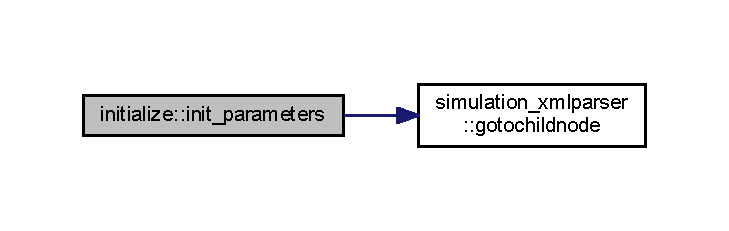
\includegraphics[width=350pt]{namespaceinitialize_a7a54dc126f448bea2b566339a449f85c_cgraph}
\end{center}
\end{figure}
Here is the caller graph for this function\+:
\nopagebreak
\begin{figure}[H]
\begin{center}
\leavevmode
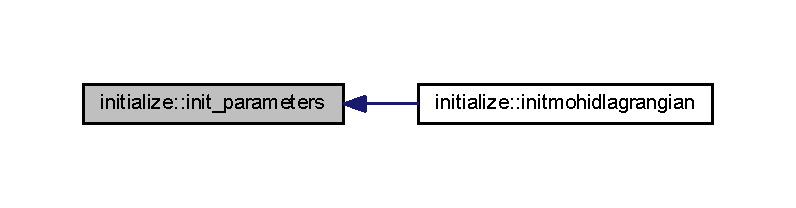
\includegraphics[width=350pt]{namespaceinitialize_a7a54dc126f448bea2b566339a449f85c_icgraph}
\end{center}
\end{figure}
\mbox{\Hypertarget{namespaceinitialize_a4640ad15e29b88467ec842f274f64b62}\label{namespaceinitialize_a4640ad15e29b88467ec842f274f64b62}} 
\index{initialize@{initialize}!init\+\_\+properties@{init\+\_\+properties}}
\index{init\+\_\+properties@{init\+\_\+properties}!initialize@{initialize}}
\subsubsection{\texorpdfstring{init\+\_\+properties()}{init\_properties()}}
{\footnotesize\ttfamily subroutine initialize\+::init\+\_\+properties (\begin{DoxyParamCaption}\item[{type(node), intent(in), pointer}]{case\+\_\+node }\end{DoxyParamCaption})\hspace{0.3cm}{\ttfamily [private]}}



Birjukovs Canelas -\/ M\+A\+R\+E\+T\+EC 

Private property xml parser routine. Reads the properties tab from the xml file and links these to the corresponding source 
\begin{DoxyParams}[1]{Parameters}
\mbox{\tt in}  & {\em parsedxml} & \\
\hline
\end{DoxyParams}
Here is the call graph for this function\+:
\nopagebreak
\begin{figure}[H]
\begin{center}
\leavevmode
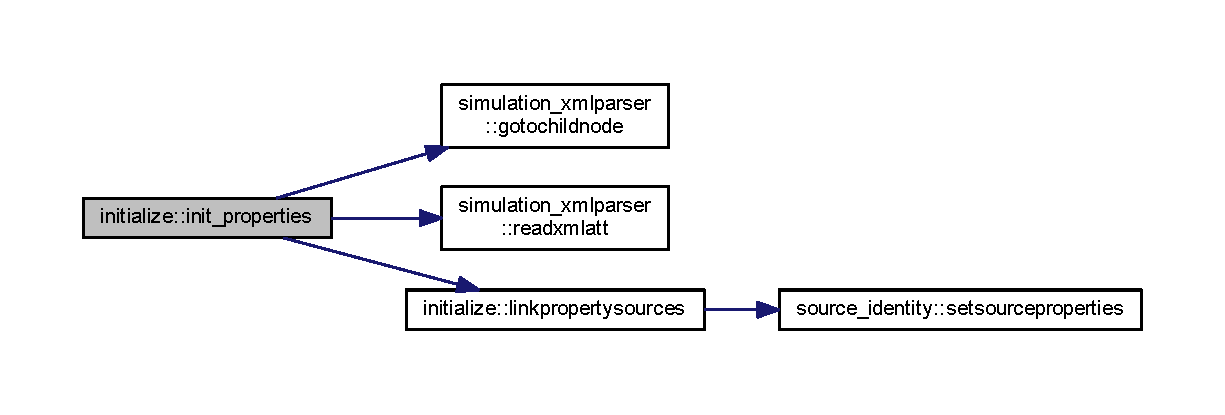
\includegraphics[width=350pt]{namespaceinitialize_a4640ad15e29b88467ec842f274f64b62_cgraph}
\end{center}
\end{figure}
Here is the caller graph for this function\+:
\nopagebreak
\begin{figure}[H]
\begin{center}
\leavevmode
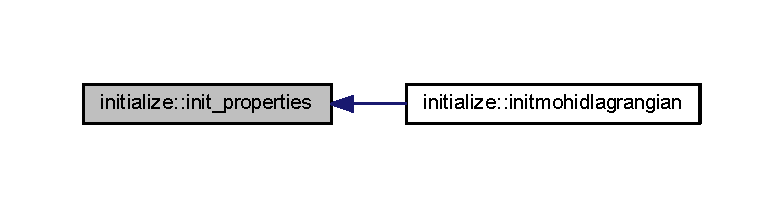
\includegraphics[width=350pt]{namespaceinitialize_a4640ad15e29b88467ec842f274f64b62_icgraph}
\end{center}
\end{figure}
\mbox{\Hypertarget{namespaceinitialize_adb972e92da4789506ee6b62b702df2b3}\label{namespaceinitialize_adb972e92da4789506ee6b62b702df2b3}} 
\index{initialize@{initialize}!init\+\_\+simdefs@{init\+\_\+simdefs}}
\index{init\+\_\+simdefs@{init\+\_\+simdefs}!initialize@{initialize}}
\subsubsection{\texorpdfstring{init\+\_\+simdefs()}{init\_simdefs()}}
{\footnotesize\ttfamily subroutine initialize\+::init\+\_\+simdefs (\begin{DoxyParamCaption}\item[{type(node), intent(in), pointer}]{case\+\_\+node }\end{DoxyParamCaption})\hspace{0.3cm}{\ttfamily [private]}}



Birjukovs Canelas -\/ M\+A\+R\+E\+T\+EC 

Private simulation definitions parser routine. Builds the simulation geometric space from the input xml case file. 
\begin{DoxyParams}[1]{Parameters}
\mbox{\tt in}  & {\em parsedxml} & \\
\hline
\end{DoxyParams}
Here is the call graph for this function\+:
\nopagebreak
\begin{figure}[H]
\begin{center}
\leavevmode
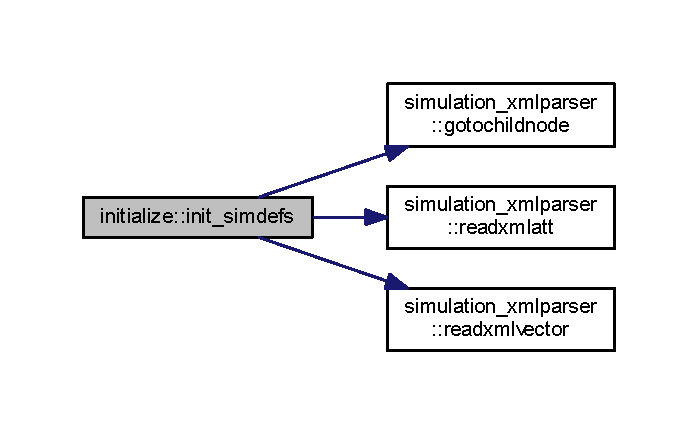
\includegraphics[width=335pt]{namespaceinitialize_adb972e92da4789506ee6b62b702df2b3_cgraph}
\end{center}
\end{figure}
Here is the caller graph for this function\+:
\nopagebreak
\begin{figure}[H]
\begin{center}
\leavevmode
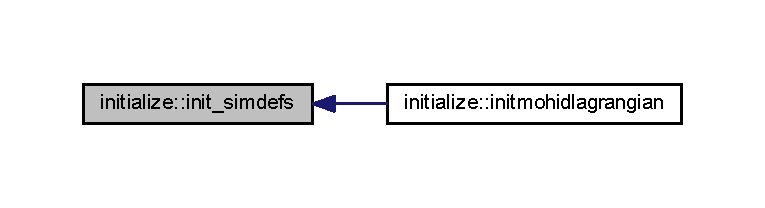
\includegraphics[width=350pt]{namespaceinitialize_adb972e92da4789506ee6b62b702df2b3_icgraph}
\end{center}
\end{figure}
\mbox{\Hypertarget{namespaceinitialize_a9ed75476e5dd07928aed3442281930be}\label{namespaceinitialize_a9ed75476e5dd07928aed3442281930be}} 
\index{initialize@{initialize}!init\+\_\+sources@{init\+\_\+sources}}
\index{init\+\_\+sources@{init\+\_\+sources}!initialize@{initialize}}
\subsubsection{\texorpdfstring{init\+\_\+sources()}{init\_sources()}}
{\footnotesize\ttfamily subroutine initialize\+::init\+\_\+sources (\begin{DoxyParamCaption}\item[{type(node), intent(in), pointer}]{case\+\_\+node }\end{DoxyParamCaption})\hspace{0.3cm}{\ttfamily [private]}}



Birjukovs Canelas -\/ M\+A\+R\+E\+T\+EC 

Private source definitions parser routine. Builds the tracer sources from the input xml case file. 
\begin{DoxyParams}[1]{Parameters}
\mbox{\tt in}  & {\em parsedxml} & \\
\hline
\end{DoxyParams}
Here is the call graph for this function\+:
\nopagebreak
\begin{figure}[H]
\begin{center}
\leavevmode
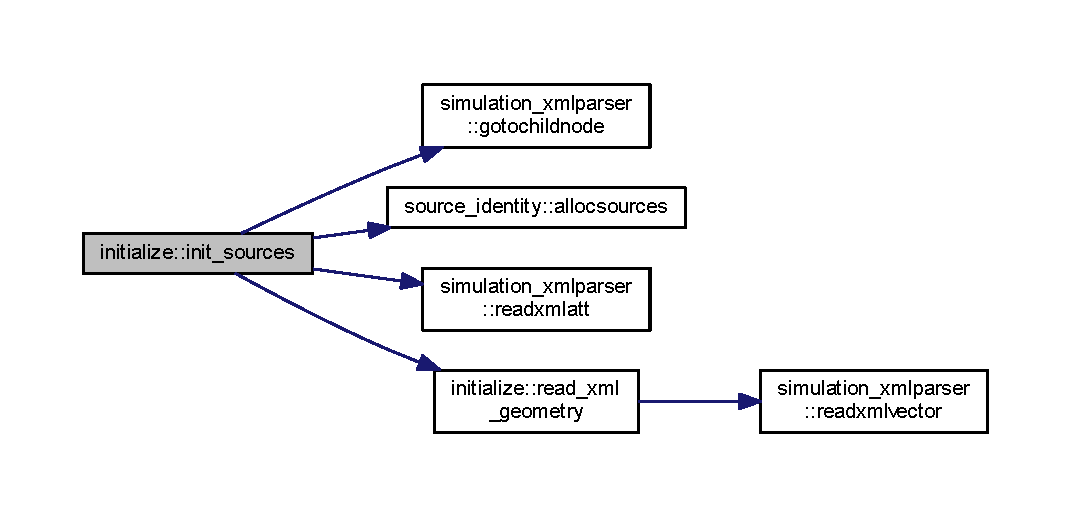
\includegraphics[width=350pt]{namespaceinitialize_a9ed75476e5dd07928aed3442281930be_cgraph}
\end{center}
\end{figure}
Here is the caller graph for this function\+:
\nopagebreak
\begin{figure}[H]
\begin{center}
\leavevmode
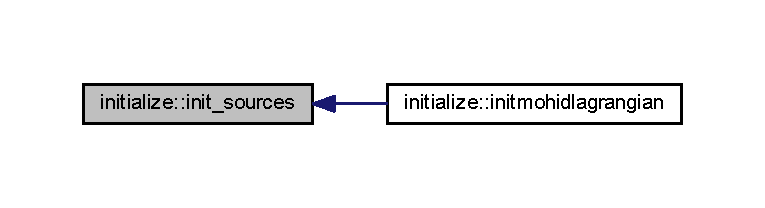
\includegraphics[width=350pt]{namespaceinitialize_a9ed75476e5dd07928aed3442281930be_icgraph}
\end{center}
\end{figure}
\mbox{\Hypertarget{namespaceinitialize_a45b7ca20c45cf272acbc391950cbb804}\label{namespaceinitialize_a45b7ca20c45cf272acbc391950cbb804}} 
\index{initialize@{initialize}!initmohidlagrangian@{initmohidlagrangian}}
\index{initmohidlagrangian@{initmohidlagrangian}!initialize@{initialize}}
\subsubsection{\texorpdfstring{initmohidlagrangian()}{initmohidlagrangian()}}
{\footnotesize\ttfamily subroutine, public initialize\+::initmohidlagrangian (\begin{DoxyParamCaption}\item[{type(string), intent(in)}]{xmlfilename }\end{DoxyParamCaption})}



Birjukovs Canelas -\/ M\+A\+R\+E\+T\+EC 

Public xml parser routine. Builds the simulation space from the input xml case file. 
\begin{DoxyParams}[1]{Parameters}
\mbox{\tt in}  & {\em xmlfilename} & \\
\hline
\mbox{\tt in}  & {\em xmlfilename} & .xml file name \\
\hline
\end{DoxyParams}
Here is the call graph for this function\+:
\nopagebreak
\begin{figure}[H]
\begin{center}
\leavevmode
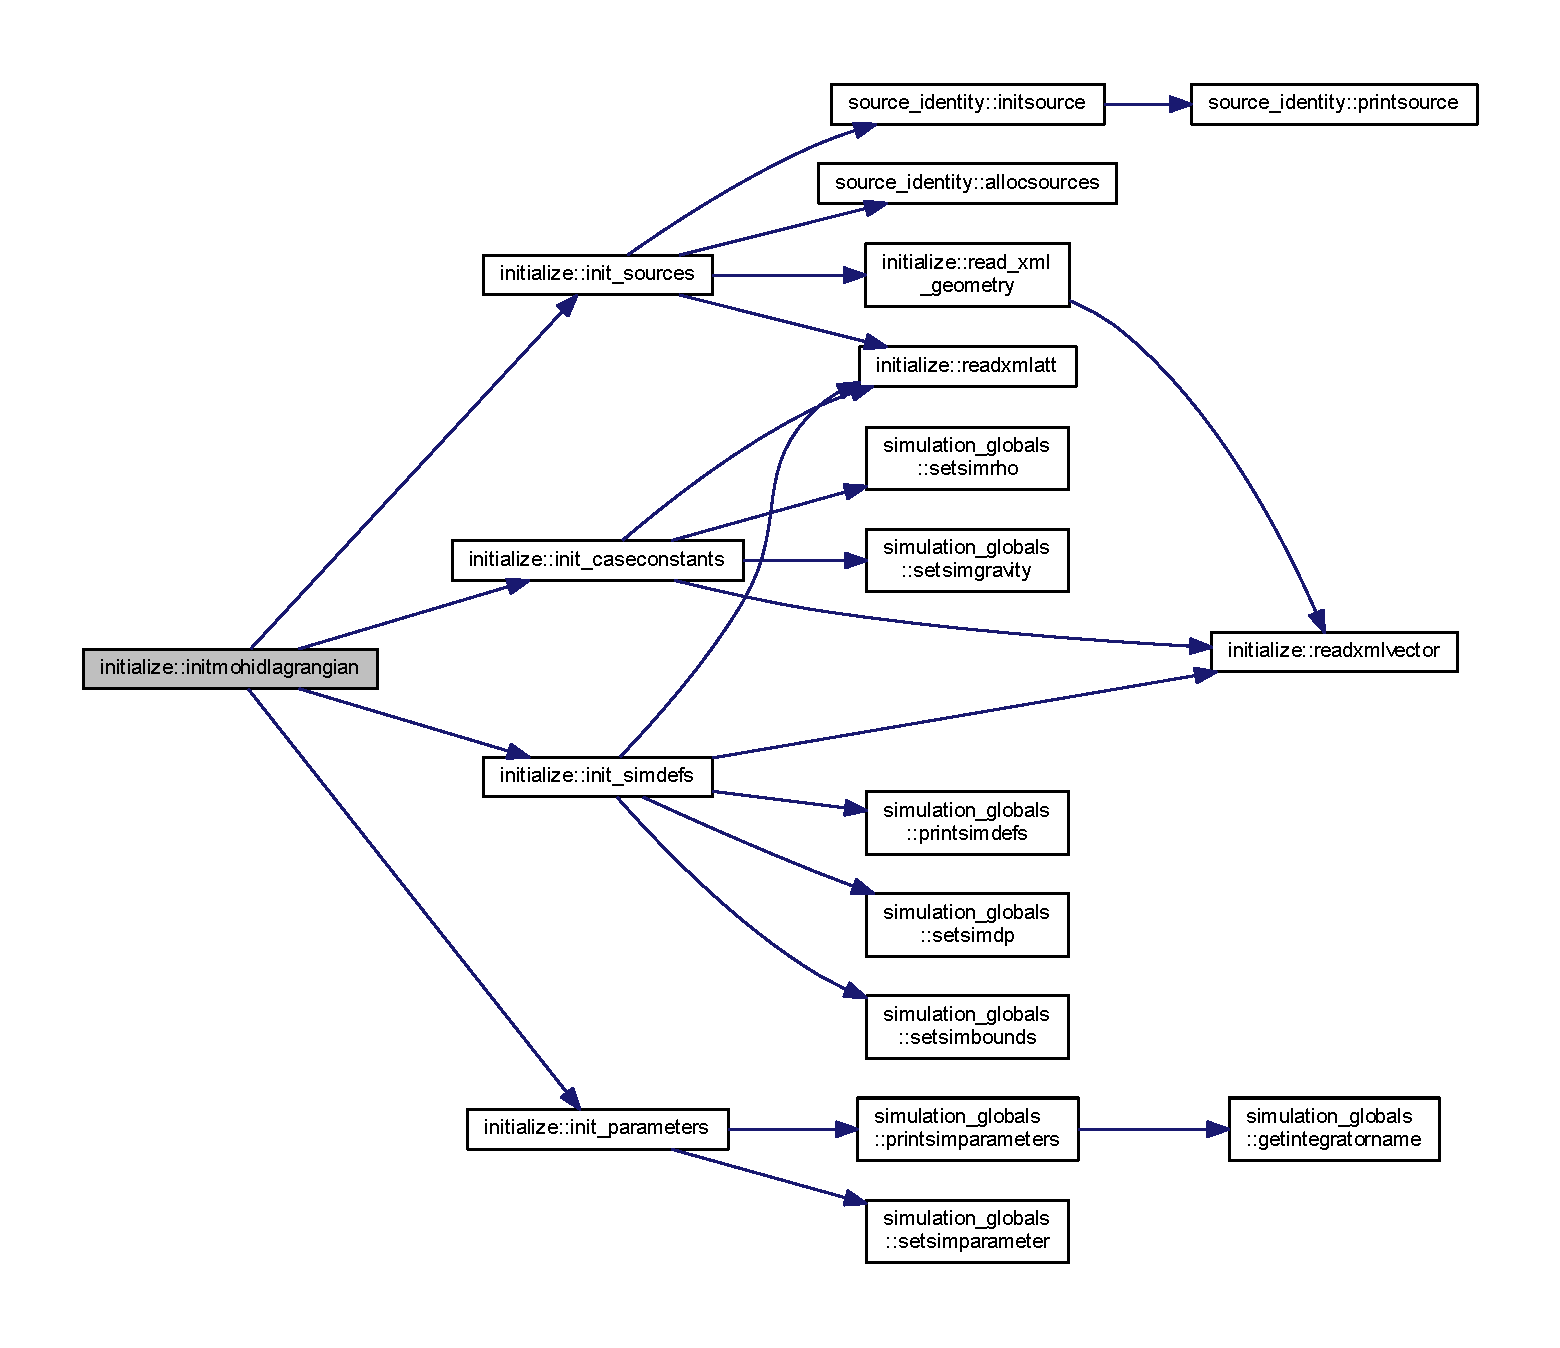
\includegraphics[width=350pt]{namespaceinitialize_a45b7ca20c45cf272acbc391950cbb804_cgraph}
\end{center}
\end{figure}
\mbox{\Hypertarget{namespaceinitialize_ab91b27efd537a161ee9ca4b2d9efde1a}\label{namespaceinitialize_ab91b27efd537a161ee9ca4b2d9efde1a}} 
\index{initialize@{initialize}!linkpropertysources@{linkpropertysources}}
\index{linkpropertysources@{linkpropertysources}!initialize@{initialize}}
\subsubsection{\texorpdfstring{linkpropertysources()}{linkpropertysources()}}
{\footnotesize\ttfamily subroutine initialize\+::linkpropertysources (\begin{DoxyParamCaption}\item[{type(node), intent(in), pointer}]{links\+Node }\end{DoxyParamCaption})\hspace{0.3cm}{\ttfamily [private]}}



Birjukovs Canelas -\/ M\+A\+R\+E\+T\+EC 

Private property xml parser routine. Reads the properties tab from the xml file and links these to the corresponding source 
\begin{DoxyParams}[1]{Parameters}
\mbox{\tt in}  & {\em parsedxml} & \\
\hline
\end{DoxyParams}
Here is the call graph for this function\+:
\nopagebreak
\begin{figure}[H]
\begin{center}
\leavevmode
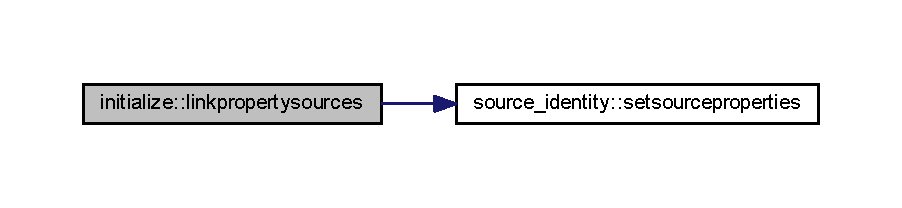
\includegraphics[width=350pt]{namespaceinitialize_ab91b27efd537a161ee9ca4b2d9efde1a_cgraph}
\end{center}
\end{figure}
Here is the caller graph for this function\+:
\nopagebreak
\begin{figure}[H]
\begin{center}
\leavevmode
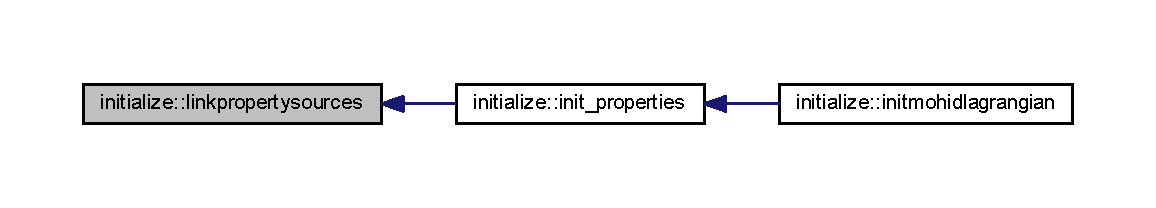
\includegraphics[width=350pt]{namespaceinitialize_ab91b27efd537a161ee9ca4b2d9efde1a_icgraph}
\end{center}
\end{figure}
\mbox{\Hypertarget{namespaceinitialize_ad36e4f602dab66c06a1f0e2474e9f0a6}\label{namespaceinitialize_ad36e4f602dab66c06a1f0e2474e9f0a6}} 
\index{initialize@{initialize}!read\+\_\+xml\+\_\+geometry@{read\+\_\+xml\+\_\+geometry}}
\index{read\+\_\+xml\+\_\+geometry@{read\+\_\+xml\+\_\+geometry}!initialize@{initialize}}
\subsubsection{\texorpdfstring{read\+\_\+xml\+\_\+geometry()}{read\_xml\_geometry()}}
{\footnotesize\ttfamily subroutine initialize\+::read\+\_\+xml\+\_\+geometry (\begin{DoxyParamCaption}\item[{type(node), intent(in), pointer}]{source,  }\item[{type(node), intent(in), pointer}]{source\+\_\+detail,  }\item[{class(\mbox{\hyperlink{structgeometry_1_1shape}{shape}}), intent(inout)}]{geometry }\end{DoxyParamCaption})\hspace{0.3cm}{\ttfamily [private]}}



Birjukovs Canelas -\/ M\+A\+R\+E\+T\+EC 

Private geometry xml parser routine. Reads a geometry from the xml depending on the geometry type of the node 
\begin{DoxyParams}[1]{Parameters}
\mbox{\tt in}  & {\em source,geometry} & \\
\hline
\mbox{\tt in}  & {\em source} & Working xml node\\
\hline
\mbox{\tt in}  & {\em source\+\_\+detail} & Working xml node details\\
\hline
\mbox{\tt in,out}  & {\em geometry} & Geometrical object to fill \\
\hline
\end{DoxyParams}
Here is the call graph for this function\+:
\nopagebreak
\begin{figure}[H]
\begin{center}
\leavevmode
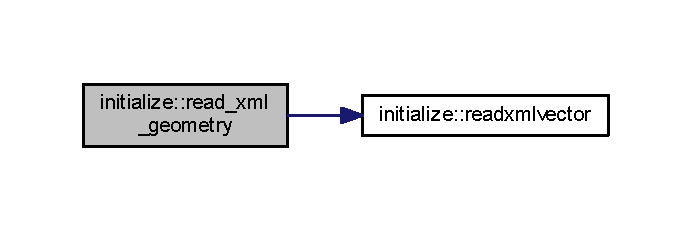
\includegraphics[width=323pt]{namespaceinitialize_ad36e4f602dab66c06a1f0e2474e9f0a6_cgraph}
\end{center}
\end{figure}
Here is the caller graph for this function\+:
\nopagebreak
\begin{figure}[H]
\begin{center}
\leavevmode
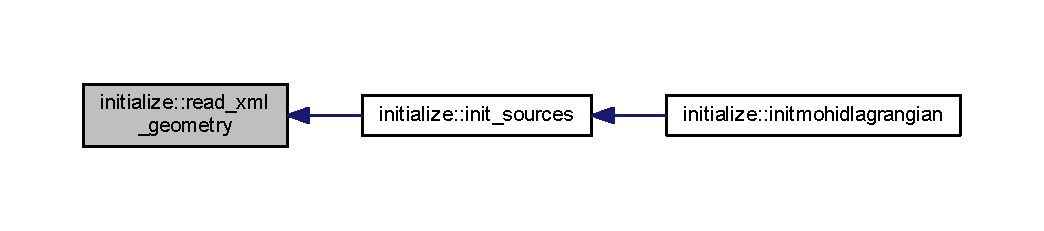
\includegraphics[width=350pt]{namespaceinitialize_ad36e4f602dab66c06a1f0e2474e9f0a6_icgraph}
\end{center}
\end{figure}

\hypertarget{namespacesimulation__parameters}{}\section{simulation\+\_\+parameters Module Reference}
\label{namespacesimulation__parameters}\index{simulation\+\_\+parameters@{simulation\+\_\+parameters}}


Module to hold all the simulation related parameters, definitions and methods.  


\subsection*{Functions/\+Subroutines}
\begin{DoxyCompactItemize}
\item 
subroutine, public \mbox{\hyperlink{namespacesimulation__parameters_af905a4701f68f0ad0a50606101fda7d6}{setsimparameter}} (parmkey, parmvalue)
\begin{DoxyCompactList}\small\item\em Birjukovs Canelas -\/ M\+A\+R\+E\+T\+EC \end{DoxyCompactList}\item 
subroutine, public \mbox{\hyperlink{namespacesimulation__parameters_a21b04e29ccee801263abc6e27fba026f}{setsimgravity}} (grav)
\begin{DoxyCompactList}\small\item\em Birjukovs Canelas -\/ M\+A\+R\+E\+T\+EC \end{DoxyCompactList}\item 
subroutine, public \mbox{\hyperlink{namespacesimulation__parameters_a877176f5e4ba2c41a2514b824520f315}{setsimrho}} (read\+\_\+rho)
\begin{DoxyCompactList}\small\item\em Birjukovs Canelas -\/ M\+A\+R\+E\+T\+EC \end{DoxyCompactList}\item 
subroutine, public \mbox{\hyperlink{namespacesimulation__parameters_a757c1773e1c21deb9f3bfd2dc258bd1a}{setsimdp}} (read\+\_\+dp)
\begin{DoxyCompactList}\small\item\em Birjukovs Canelas -\/ M\+A\+R\+E\+T\+EC \end{DoxyCompactList}\item 
subroutine, public \mbox{\hyperlink{namespacesimulation__parameters_a71f285f54b412efac79d40c9ecd58037}{setsimbounds}} (point\+\_\+, coords)
\begin{DoxyCompactList}\small\item\em Birjukovs Canelas -\/ M\+A\+R\+E\+T\+EC \end{DoxyCompactList}\end{DoxyCompactItemize}
\subsection*{Variables}
\begin{DoxyCompactItemize}
\item 
integer, public \mbox{\hyperlink{namespacesimulation__parameters_a0a398ad974eef004e43a347105e8ad81}{integrator}} = 1
\item 
real(prec), public \mbox{\hyperlink{namespacesimulation__parameters_a82ce5585265987eedbbaad0cd9cac673}{cfl}} = 0.\+5
\item 
real(prec), public \mbox{\hyperlink{namespacesimulation__parameters_add65346bea9045d3ea4573be190f7cdc}{initfreeze}} = 0.\+0
\item 
real(prec), public \mbox{\hyperlink{namespacesimulation__parameters_aedd90d7d1a6db61fcac836ac37034e75}{timemax}} = MV
\item 
real(prec), public \mbox{\hyperlink{namespacesimulation__parameters_a70ee14718c33544ce34bf7990211e5cc}{timeout}} = MV
\item 
real(prec), public \mbox{\hyperlink{namespacesimulation__parameters_afe85a1735413a2cc7a220910f68bd214}{dp}} = MV
\item 
type(vector), public \mbox{\hyperlink{namespacesimulation__parameters_acb9016ab495389a3b970541d9ec585cf}{pointmin}}
\item 
type(vector), public \mbox{\hyperlink{namespacesimulation__parameters_ac8471983089d031118d18a4b498d4e0d}{pointmax}}
\item 
type(vector), public \mbox{\hyperlink{namespacesimulation__parameters_a5f4b25aae7394e93796760f8720af525}{gravity}}
\item 
real(prec), public \mbox{\hyperlink{namespacesimulation__parameters_afde4a9da604d884c51389f6fa871e521}{rho\+\_\+ref}} = 1000.\+0
\end{DoxyCompactItemize}


\subsection{Detailed Description}
Module to hold all the simulation related parameters, definitions and methods. 

\begin{DoxyAuthor}{Author}
Ricardo Birjukovs Canelas 
\end{DoxyAuthor}


\subsection{Function/\+Subroutine Documentation}
\mbox{\Hypertarget{namespacesimulation__parameters_a71f285f54b412efac79d40c9ecd58037}\label{namespacesimulation__parameters_a71f285f54b412efac79d40c9ecd58037}} 
\index{simulation\+\_\+parameters@{simulation\+\_\+parameters}!setsimbounds@{setsimbounds}}
\index{setsimbounds@{setsimbounds}!simulation\+\_\+parameters@{simulation\+\_\+parameters}}
\subsubsection{\texorpdfstring{setsimbounds()}{setsimbounds()}}
{\footnotesize\ttfamily subroutine, public simulation\+\_\+parameters\+::setsimbounds (\begin{DoxyParamCaption}\item[{type(string), intent(in)}]{point\+\_\+,  }\item[{type(vector)}]{coords }\end{DoxyParamCaption})}



Birjukovs Canelas -\/ M\+A\+R\+E\+T\+EC 

Public bounding box setting routine. 
\begin{DoxyParams}[1]{Parameters}
\mbox{\tt in}  & {\em point\+\_\+,coords} & \\
\hline
\end{DoxyParams}
\mbox{\Hypertarget{namespacesimulation__parameters_a757c1773e1c21deb9f3bfd2dc258bd1a}\label{namespacesimulation__parameters_a757c1773e1c21deb9f3bfd2dc258bd1a}} 
\index{simulation\+\_\+parameters@{simulation\+\_\+parameters}!setsimdp@{setsimdp}}
\index{setsimdp@{setsimdp}!simulation\+\_\+parameters@{simulation\+\_\+parameters}}
\subsubsection{\texorpdfstring{setsimdp()}{setsimdp()}}
{\footnotesize\ttfamily subroutine, public simulation\+\_\+parameters\+::setsimdp (\begin{DoxyParamCaption}\item[{type(string), intent(in)}]{read\+\_\+dp }\end{DoxyParamCaption})}



Birjukovs Canelas -\/ M\+A\+R\+E\+T\+EC 

Public dp setting routine. 
\begin{DoxyParams}[1]{Parameters}
\mbox{\tt in}  & {\em read\+\_\+dp} & \\
\hline
\end{DoxyParams}
\mbox{\Hypertarget{namespacesimulation__parameters_a21b04e29ccee801263abc6e27fba026f}\label{namespacesimulation__parameters_a21b04e29ccee801263abc6e27fba026f}} 
\index{simulation\+\_\+parameters@{simulation\+\_\+parameters}!setsimgravity@{setsimgravity}}
\index{setsimgravity@{setsimgravity}!simulation\+\_\+parameters@{simulation\+\_\+parameters}}
\subsubsection{\texorpdfstring{setsimgravity()}{setsimgravity()}}
{\footnotesize\ttfamily subroutine, public simulation\+\_\+parameters\+::setsimgravity (\begin{DoxyParamCaption}\item[{type(vector)}]{grav }\end{DoxyParamCaption})}



Birjukovs Canelas -\/ M\+A\+R\+E\+T\+EC 

Public Gravity setting routine. 
\begin{DoxyParams}[1]{Parameters}
\mbox{\tt in}  & {\em grav} & \\
\hline
\end{DoxyParams}
\mbox{\Hypertarget{namespacesimulation__parameters_af905a4701f68f0ad0a50606101fda7d6}\label{namespacesimulation__parameters_af905a4701f68f0ad0a50606101fda7d6}} 
\index{simulation\+\_\+parameters@{simulation\+\_\+parameters}!setsimparameter@{setsimparameter}}
\index{setsimparameter@{setsimparameter}!simulation\+\_\+parameters@{simulation\+\_\+parameters}}
\subsubsection{\texorpdfstring{setsimparameter()}{setsimparameter()}}
{\footnotesize\ttfamily subroutine, public simulation\+\_\+parameters\+::setsimparameter (\begin{DoxyParamCaption}\item[{type(string), intent(in)}]{parmkey,  }\item[{type(string), intent(in)}]{parmvalue }\end{DoxyParamCaption})}



Birjukovs Canelas -\/ M\+A\+R\+E\+T\+EC 

Public parameter setting routine. Builds the simulation parametric space from the input xml case file. 
\begin{DoxyParams}[1]{Parameters}
\mbox{\tt in}  & {\em parmkey} & \\
\hline
\mbox{\tt in}  & {\em parmvalue} & \\
\hline
\end{DoxyParams}
\mbox{\Hypertarget{namespacesimulation__parameters_a877176f5e4ba2c41a2514b824520f315}\label{namespacesimulation__parameters_a877176f5e4ba2c41a2514b824520f315}} 
\index{simulation\+\_\+parameters@{simulation\+\_\+parameters}!setsimrho@{setsimrho}}
\index{setsimrho@{setsimrho}!simulation\+\_\+parameters@{simulation\+\_\+parameters}}
\subsubsection{\texorpdfstring{setsimrho()}{setsimrho()}}
{\footnotesize\ttfamily subroutine, public simulation\+\_\+parameters\+::setsimrho (\begin{DoxyParamCaption}\item[{type(string), intent(in)}]{read\+\_\+rho }\end{DoxyParamCaption})}



Birjukovs Canelas -\/ M\+A\+R\+E\+T\+EC 

Public Rho\+\_\+\+Ref setting routine. 
\begin{DoxyParams}[1]{Parameters}
\mbox{\tt in}  & {\em rho} & \\
\hline
\end{DoxyParams}


\subsection{Variable Documentation}
\mbox{\Hypertarget{namespacesimulation__parameters_a82ce5585265987eedbbaad0cd9cac673}\label{namespacesimulation__parameters_a82ce5585265987eedbbaad0cd9cac673}} 
\index{simulation\+\_\+parameters@{simulation\+\_\+parameters}!cfl@{cfl}}
\index{cfl@{cfl}!simulation\+\_\+parameters@{simulation\+\_\+parameters}}
\subsubsection{\texorpdfstring{cfl}{cfl}}
{\footnotesize\ttfamily real(prec), public simulation\+\_\+parameters\+::cfl = 0.\+5}

\mbox{\Hypertarget{namespacesimulation__parameters_afe85a1735413a2cc7a220910f68bd214}\label{namespacesimulation__parameters_afe85a1735413a2cc7a220910f68bd214}} 
\index{simulation\+\_\+parameters@{simulation\+\_\+parameters}!dp@{dp}}
\index{dp@{dp}!simulation\+\_\+parameters@{simulation\+\_\+parameters}}
\subsubsection{\texorpdfstring{dp}{dp}}
{\footnotesize\ttfamily real(prec), public simulation\+\_\+parameters\+::dp = MV}

\mbox{\Hypertarget{namespacesimulation__parameters_a5f4b25aae7394e93796760f8720af525}\label{namespacesimulation__parameters_a5f4b25aae7394e93796760f8720af525}} 
\index{simulation\+\_\+parameters@{simulation\+\_\+parameters}!gravity@{gravity}}
\index{gravity@{gravity}!simulation\+\_\+parameters@{simulation\+\_\+parameters}}
\subsubsection{\texorpdfstring{gravity}{gravity}}
{\footnotesize\ttfamily type(vector), public simulation\+\_\+parameters\+::gravity}

\mbox{\Hypertarget{namespacesimulation__parameters_add65346bea9045d3ea4573be190f7cdc}\label{namespacesimulation__parameters_add65346bea9045d3ea4573be190f7cdc}} 
\index{simulation\+\_\+parameters@{simulation\+\_\+parameters}!initfreeze@{initfreeze}}
\index{initfreeze@{initfreeze}!simulation\+\_\+parameters@{simulation\+\_\+parameters}}
\subsubsection{\texorpdfstring{initfreeze}{initfreeze}}
{\footnotesize\ttfamily real(prec), public simulation\+\_\+parameters\+::initfreeze = 0.\+0}

\mbox{\Hypertarget{namespacesimulation__parameters_a0a398ad974eef004e43a347105e8ad81}\label{namespacesimulation__parameters_a0a398ad974eef004e43a347105e8ad81}} 
\index{simulation\+\_\+parameters@{simulation\+\_\+parameters}!integrator@{integrator}}
\index{integrator@{integrator}!simulation\+\_\+parameters@{simulation\+\_\+parameters}}
\subsubsection{\texorpdfstring{integrator}{integrator}}
{\footnotesize\ttfamily integer, public simulation\+\_\+parameters\+::integrator = 1}

\mbox{\Hypertarget{namespacesimulation__parameters_ac8471983089d031118d18a4b498d4e0d}\label{namespacesimulation__parameters_ac8471983089d031118d18a4b498d4e0d}} 
\index{simulation\+\_\+parameters@{simulation\+\_\+parameters}!pointmax@{pointmax}}
\index{pointmax@{pointmax}!simulation\+\_\+parameters@{simulation\+\_\+parameters}}
\subsubsection{\texorpdfstring{pointmax}{pointmax}}
{\footnotesize\ttfamily type(vector), public simulation\+\_\+parameters\+::pointmax}

\mbox{\Hypertarget{namespacesimulation__parameters_acb9016ab495389a3b970541d9ec585cf}\label{namespacesimulation__parameters_acb9016ab495389a3b970541d9ec585cf}} 
\index{simulation\+\_\+parameters@{simulation\+\_\+parameters}!pointmin@{pointmin}}
\index{pointmin@{pointmin}!simulation\+\_\+parameters@{simulation\+\_\+parameters}}
\subsubsection{\texorpdfstring{pointmin}{pointmin}}
{\footnotesize\ttfamily type(vector), public simulation\+\_\+parameters\+::pointmin}

\mbox{\Hypertarget{namespacesimulation__parameters_afde4a9da604d884c51389f6fa871e521}\label{namespacesimulation__parameters_afde4a9da604d884c51389f6fa871e521}} 
\index{simulation\+\_\+parameters@{simulation\+\_\+parameters}!rho\+\_\+ref@{rho\+\_\+ref}}
\index{rho\+\_\+ref@{rho\+\_\+ref}!simulation\+\_\+parameters@{simulation\+\_\+parameters}}
\subsubsection{\texorpdfstring{rho\+\_\+ref}{rho\_ref}}
{\footnotesize\ttfamily real(prec), public simulation\+\_\+parameters\+::rho\+\_\+ref = 1000.\+0}

\mbox{\Hypertarget{namespacesimulation__parameters_aedd90d7d1a6db61fcac836ac37034e75}\label{namespacesimulation__parameters_aedd90d7d1a6db61fcac836ac37034e75}} 
\index{simulation\+\_\+parameters@{simulation\+\_\+parameters}!timemax@{timemax}}
\index{timemax@{timemax}!simulation\+\_\+parameters@{simulation\+\_\+parameters}}
\subsubsection{\texorpdfstring{timemax}{timemax}}
{\footnotesize\ttfamily real(prec), public simulation\+\_\+parameters\+::timemax = MV}

\mbox{\Hypertarget{namespacesimulation__parameters_a70ee14718c33544ce34bf7990211e5cc}\label{namespacesimulation__parameters_a70ee14718c33544ce34bf7990211e5cc}} 
\index{simulation\+\_\+parameters@{simulation\+\_\+parameters}!timeout@{timeout}}
\index{timeout@{timeout}!simulation\+\_\+parameters@{simulation\+\_\+parameters}}
\subsubsection{\texorpdfstring{timeout}{timeout}}
{\footnotesize\ttfamily real(prec), public simulation\+\_\+parameters\+::timeout = MV}


\hypertarget{namespacesource}{}\section{source Module Reference}
\label{namespacesource}\index{source@{source}}


Module to hold and wrap all the tracer sources respective modules. Defines a source class and related methods.  




\subsection{Detailed Description}
Module to hold and wrap all the tracer sources respective modules. Defines a source class and related methods. 

\begin{DoxyAuthor}{Author}
Ricardo Birjukovs Canelas 
\end{DoxyAuthor}

\hypertarget{namespacesource__emitter}{}\section{source\+\_\+emitter Module Reference}
\label{namespacesource__emitter}\index{source\+\_\+emitter@{source\+\_\+emitter}}


Module that defines an emitter class and related methods. This module is responsible for building a potential tracer list based on the availble sources and calling their initializers.  


\subsection*{Data Types}
\begin{DoxyCompactItemize}
\item 
type \mbox{\hyperlink{structsource__emitter_1_1emitter__t}{emitter\+\_\+t}}
\end{DoxyCompactItemize}
\subsection*{Functions/\+Subroutines}
\begin{DoxyCompactItemize}
\item 
subroutine \mbox{\hyperlink{namespacesource__emitter_a18e5a215687e0f5f13c0148be0f0c0e6}{initialize}} (self, srcs, nsrcs)
\begin{DoxyCompactList}\small\item\em Birjukovs Canelas -\/ M\+A\+R\+E\+T\+EC \end{DoxyCompactList}\item 
subroutine \mbox{\hyperlink{namespacesource__emitter_a73d054a39fc1fccfde74173a5c7f2c58}{setotalnp}} (src)
\begin{DoxyCompactList}\small\item\em Birjukovs Canelas -\/ M\+A\+R\+E\+T\+EC \end{DoxyCompactList}\end{DoxyCompactItemize}
\subsection*{Variables}
\begin{DoxyCompactItemize}
\item 
type(\mbox{\hyperlink{structsource__emitter_1_1emitter__t}{emitter\+\_\+t}}), public \mbox{\hyperlink{namespacesource__emitter_a357876a84a74e23c44e92ab8ef7dc35e}{emitter}}
\end{DoxyCompactItemize}


\subsection{Detailed Description}
Module that defines an emitter class and related methods. This module is responsible for building a potential tracer list based on the availble sources and calling their initializers. 

\begin{DoxyAuthor}{Author}
Ricardo Birjukovs Canelas 
\end{DoxyAuthor}


\subsection{Function/\+Subroutine Documentation}
\mbox{\Hypertarget{namespacesource__emitter_a18e5a215687e0f5f13c0148be0f0c0e6}\label{namespacesource__emitter_a18e5a215687e0f5f13c0148be0f0c0e6}} 
\index{source\+\_\+emitter@{source\+\_\+emitter}!initialize@{initialize}}
\index{initialize@{initialize}!source\+\_\+emitter@{source\+\_\+emitter}}
\subsubsection{\texorpdfstring{initialize()}{initialize()}}
{\footnotesize\ttfamily subroutine source\+\_\+emitter\+::initialize (\begin{DoxyParamCaption}\item[{class(\mbox{\hyperlink{structsource__emitter_1_1emitter__t}{emitter\+\_\+t}}), intent(in)}]{self,  }\item[{class(\mbox{\hyperlink{structsource__identity_1_1source__class}{source\+\_\+class}}), dimension(nsrcs), intent(inout)}]{srcs,  }\item[{integer, intent(in)}]{nsrcs }\end{DoxyParamCaption})\hspace{0.3cm}{\ttfamily [private]}}



Birjukovs Canelas -\/ M\+A\+R\+E\+T\+EC 

method that returns the total number of tracers an input source can potentially create 
\begin{DoxyParams}[1]{Parameters}
\mbox{\tt in}  & {\em self,src} & \\
\hline
\end{DoxyParams}
Here is the call graph for this function\+:\nopagebreak
\begin{figure}[H]
\begin{center}
\leavevmode
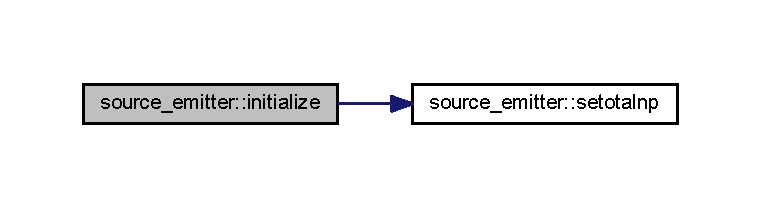
\includegraphics[width=350pt]{namespacesource__emitter_a18e5a215687e0f5f13c0148be0f0c0e6_cgraph}
\end{center}
\end{figure}
\mbox{\Hypertarget{namespacesource__emitter_a73d054a39fc1fccfde74173a5c7f2c58}\label{namespacesource__emitter_a73d054a39fc1fccfde74173a5c7f2c58}} 
\index{source\+\_\+emitter@{source\+\_\+emitter}!setotalnp@{setotalnp}}
\index{setotalnp@{setotalnp}!source\+\_\+emitter@{source\+\_\+emitter}}
\subsubsection{\texorpdfstring{setotalnp()}{setotalnp()}}
{\footnotesize\ttfamily subroutine source\+\_\+emitter\+::setotalnp (\begin{DoxyParamCaption}\item[{class(\mbox{\hyperlink{structsource__identity_1_1source__class}{source\+\_\+class}}), intent(inout)}]{src }\end{DoxyParamCaption})\hspace{0.3cm}{\ttfamily [private]}}



Birjukovs Canelas -\/ M\+A\+R\+E\+T\+EC 

private routine that returns the total number of tracers an input source will potentially create 
\begin{DoxyParams}[1]{Parameters}
\mbox{\tt in}  & {\em src} & \\
\hline
\end{DoxyParams}
${NP}_{total}^{source-i}=(T_{end}^{source-i}-T_{start}^{source-i})*{Rate}^{source-i}*{NP}_{emission}^{source-i}$ Here is the caller graph for this function\+:\nopagebreak
\begin{figure}[H]
\begin{center}
\leavevmode
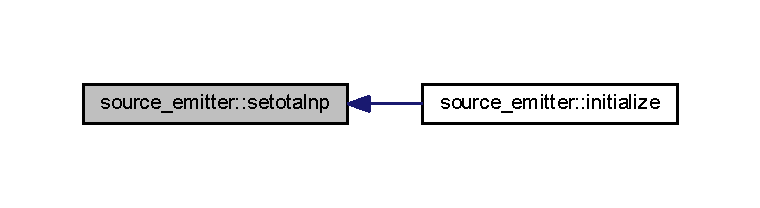
\includegraphics[width=350pt]{namespacesource__emitter_a73d054a39fc1fccfde74173a5c7f2c58_icgraph}
\end{center}
\end{figure}


\subsection{Variable Documentation}
\mbox{\Hypertarget{namespacesource__emitter_a357876a84a74e23c44e92ab8ef7dc35e}\label{namespacesource__emitter_a357876a84a74e23c44e92ab8ef7dc35e}} 
\index{source\+\_\+emitter@{source\+\_\+emitter}!emitter@{emitter}}
\index{emitter@{emitter}!source\+\_\+emitter@{source\+\_\+emitter}}
\subsubsection{\texorpdfstring{emitter}{emitter}}
{\footnotesize\ttfamily type(\mbox{\hyperlink{structsource__emitter_1_1emitter__t}{emitter\+\_\+t}}), public source\+\_\+emitter\+::emitter}


\hypertarget{namespacesource__identity}{}\section{source\+\_\+identity Module Reference}
\label{namespacesource__identity}\index{source\+\_\+identity@{source\+\_\+identity}}


Module that defines a source class and related methods.  


\subsection*{Data Types}
\begin{DoxyCompactItemize}
\item 
type \mbox{\hyperlink{structsource__identity_1_1source__class}{source\+\_\+class}}
\begin{DoxyCompactList}\small\item\em Type -\/ The source class. \end{DoxyCompactList}\item 
type \mbox{\hyperlink{structsource__identity_1_1source__par__class}{source\+\_\+par\+\_\+class}}
\item 
type \mbox{\hyperlink{structsource__identity_1_1source__state__class}{source\+\_\+state\+\_\+class}}
\begin{DoxyCompactList}\small\item\em Type -\/ state variables of a source object. \end{DoxyCompactList}\item 
type \mbox{\hyperlink{structsource__identity_1_1source__stats__class}{source\+\_\+stats\+\_\+class}}
\begin{DoxyCompactList}\small\item\em Type -\/ statistical variables of a source object. \end{DoxyCompactList}\end{DoxyCompactItemize}
\subsection*{Functions/\+Subroutines}
\begin{DoxyCompactItemize}
\item 
subroutine, public \mbox{\hyperlink{namespacesource__identity_a716b4cb4acec5756a6d4dcf20eee588e}{allocsources}} (nsources)
\begin{DoxyCompactList}\small\item\em Birjukovs Canelas -\/ M\+A\+R\+E\+T\+EC \end{DoxyCompactList}\item 
subroutine, public \mbox{\hyperlink{namespacesource__identity_a3939e59172252d0edce57e00ea41758d}{initsource}} (num, id, name, emitting\+\_\+rate, source\+\_\+geometry, geometry)
\begin{DoxyCompactList}\small\item\em Birjukovs Canelas -\/ M\+A\+R\+E\+T\+EC \end{DoxyCompactList}\item 
subroutine \mbox{\hyperlink{namespacesource__identity_ac4fc3a54de91016023a7948d261f84a5}{printsource}} (src)
\begin{DoxyCompactList}\small\item\em Birjukovs Canelas -\/ M\+A\+R\+E\+T\+EC \end{DoxyCompactList}\end{DoxyCompactItemize}
\subsection*{Variables}
\begin{DoxyCompactItemize}
\item 
type(\mbox{\hyperlink{structsource__identity_1_1source__class}{source\+\_\+class}}), dimension(\+:), allocatable, public \mbox{\hyperlink{namespacesource__identity_a5ed8006613af7461c6a2ff1cdaeb8f0f}{source}}
\end{DoxyCompactItemize}


\subsection{Detailed Description}
Module that defines a source class and related methods. 

\begin{DoxyAuthor}{Author}
Ricardo Birjukovs Canelas 
\end{DoxyAuthor}


\subsection{Function/\+Subroutine Documentation}
\mbox{\Hypertarget{namespacesource__identity_a716b4cb4acec5756a6d4dcf20eee588e}\label{namespacesource__identity_a716b4cb4acec5756a6d4dcf20eee588e}} 
\index{source\+\_\+identity@{source\+\_\+identity}!allocsources@{allocsources}}
\index{allocsources@{allocsources}!source\+\_\+identity@{source\+\_\+identity}}
\subsubsection{\texorpdfstring{allocsources()}{allocsources()}}
{\footnotesize\ttfamily subroutine, public source\+\_\+identity\+::allocsources (\begin{DoxyParamCaption}\item[{integer, intent(in)}]{nsources }\end{DoxyParamCaption})}



Birjukovs Canelas -\/ M\+A\+R\+E\+T\+EC 

source allocation routine -\/ allocates the sources objects 
\begin{DoxyParams}[1]{Parameters}
\mbox{\tt in}  & {\em nsources} & \\
\hline
\end{DoxyParams}
Here is the caller graph for this function\+:\nopagebreak
\begin{figure}[H]
\begin{center}
\leavevmode
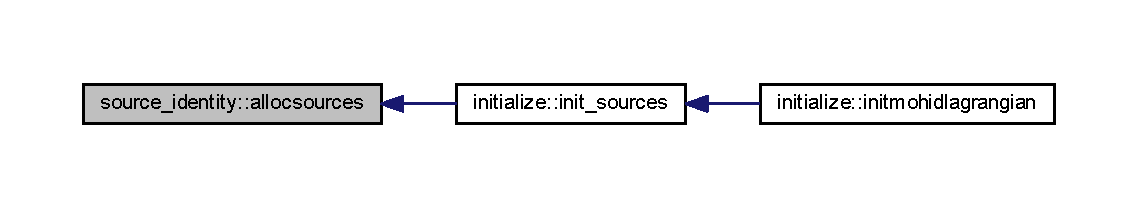
\includegraphics[width=350pt]{namespacesource__identity_a716b4cb4acec5756a6d4dcf20eee588e_icgraph}
\end{center}
\end{figure}
\mbox{\Hypertarget{namespacesource__identity_a3939e59172252d0edce57e00ea41758d}\label{namespacesource__identity_a3939e59172252d0edce57e00ea41758d}} 
\index{source\+\_\+identity@{source\+\_\+identity}!initsource@{initsource}}
\index{initsource@{initsource}!source\+\_\+identity@{source\+\_\+identity}}
\subsubsection{\texorpdfstring{initsource()}{initsource()}}
{\footnotesize\ttfamily subroutine, public source\+\_\+identity\+::initsource (\begin{DoxyParamCaption}\item[{integer, intent(in)}]{num,  }\item[{integer, intent(in)}]{id,  }\item[{type(string), intent(in)}]{name,  }\item[{real(prec), intent(in)}]{emitting\+\_\+rate,  }\item[{type(string), intent(in)}]{source\+\_\+geometry,  }\item[{class(\mbox{\hyperlink{structgeometry_1_1shape}{shape}}), intent(in)}]{geometry }\end{DoxyParamCaption})}



Birjukovs Canelas -\/ M\+A\+R\+E\+T\+EC 

source inititialization routine -\/ Generates a source and initializes its variables 
\begin{DoxyParams}[1]{Parameters}
\mbox{\tt out}  & {\em source} & \\
\hline
\mbox{\tt in}  & {\em num,id,name,emitting\+\_\+rate,source\+\_\+geometry} & \\
\hline
\end{DoxyParams}
Here is the call graph for this function\+:\nopagebreak
\begin{figure}[H]
\begin{center}
\leavevmode
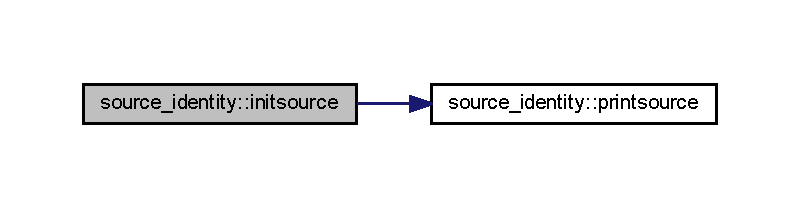
\includegraphics[width=350pt]{namespacesource__identity_a3939e59172252d0edce57e00ea41758d_cgraph}
\end{center}
\end{figure}
Here is the caller graph for this function\+:\nopagebreak
\begin{figure}[H]
\begin{center}
\leavevmode
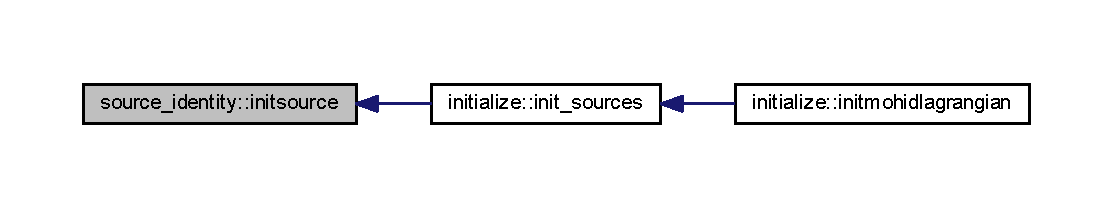
\includegraphics[width=350pt]{namespacesource__identity_a3939e59172252d0edce57e00ea41758d_icgraph}
\end{center}
\end{figure}
\mbox{\Hypertarget{namespacesource__identity_ac4fc3a54de91016023a7948d261f84a5}\label{namespacesource__identity_ac4fc3a54de91016023a7948d261f84a5}} 
\index{source\+\_\+identity@{source\+\_\+identity}!printsource@{printsource}}
\index{printsource@{printsource}!source\+\_\+identity@{source\+\_\+identity}}
\subsubsection{\texorpdfstring{printsource()}{printsource()}}
{\footnotesize\ttfamily subroutine source\+\_\+identity\+::printsource (\begin{DoxyParamCaption}\item[{type(\mbox{\hyperlink{structsource__identity_1_1source__class}{source\+\_\+class}}), intent(in)}]{src }\end{DoxyParamCaption})\hspace{0.3cm}{\ttfamily [private]}}



Birjukovs Canelas -\/ M\+A\+R\+E\+T\+EC 

source print routine -\/ prints a source info on console/log 
\begin{DoxyParams}[1]{Parameters}
\mbox{\tt in}  & {\em src} & \\
\hline
\end{DoxyParams}
Here is the caller graph for this function\+:\nopagebreak
\begin{figure}[H]
\begin{center}
\leavevmode
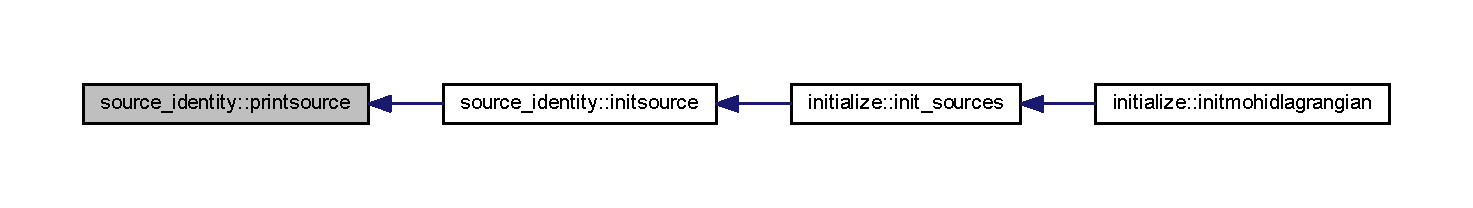
\includegraphics[width=350pt]{namespacesource__identity_ac4fc3a54de91016023a7948d261f84a5_icgraph}
\end{center}
\end{figure}


\subsection{Variable Documentation}
\mbox{\Hypertarget{namespacesource__identity_a5ed8006613af7461c6a2ff1cdaeb8f0f}\label{namespacesource__identity_a5ed8006613af7461c6a2ff1cdaeb8f0f}} 
\index{source\+\_\+identity@{source\+\_\+identity}!source@{source}}
\index{source@{source}!source\+\_\+identity@{source\+\_\+identity}}
\subsubsection{\texorpdfstring{source}{source}}
{\footnotesize\ttfamily type(\mbox{\hyperlink{structsource__identity_1_1source__class}{source\+\_\+class}}), dimension(\+:), allocatable, public source\+\_\+identity\+::source}


\hypertarget{namespacetracer}{}\section{tracer Module Reference}
\label{namespacetracer}\index{tracer@{tracer}}


Module to hold and wrap all the tracer respective modules. Defines a pure Lagrangian tracer class. This is intended to serve as the base class for every type of tracer class needed, that should be ~\newline
 built as derived of this class, with the necessary modifiers to model the desired behaviour. Basic tracer data (parameters, variables) are implemented. Tracer methods such as I/O, integration and interpolation routines are implemented.  




\subsection{Detailed Description}
Module to hold and wrap all the tracer respective modules. Defines a pure Lagrangian tracer class. This is intended to serve as the base class for every type of tracer class needed, that should be ~\newline
 built as derived of this class, with the necessary modifiers to model the desired behaviour. Basic tracer data (parameters, variables) are implemented. Tracer methods such as I/O, integration and interpolation routines are implemented. 

\begin{DoxyAuthor}{Author}
Ricardo Birjukovs Canelas 
\end{DoxyAuthor}

\hypertarget{namespacetracer2d}{}\section{tracer2d Module Reference}
\label{namespacetracer2d}\index{tracer2d@{tracer2d}}


Module that defines a pure Lagrangian 2D tracer class and related methods, as a subset of the tracer3D module.  


\subsection*{Functions/\+Subroutines}
\begin{DoxyCompactItemize}
\item 
subroutine \mbox{\hyperlink{namespacetracer2d_abebf96ac23ed37832000c68fea45f584}{tracer2d\+\_\+init}} (trc, filename, time, x, is\+\_\+sigma)
\begin{DoxyCompactList}\small\item\em Birjukovs Canelas -\/ M\+A\+R\+E\+T\+EC Routine Author Name and Affiliation. \end{DoxyCompactList}\end{DoxyCompactItemize}


\subsection{Detailed Description}
Module that defines a pure Lagrangian 2D tracer class and related methods, as a subset of the tracer3D module. 

\begin{DoxyAuthor}{Author}
Ricardo Birjukovs Canelas 
\end{DoxyAuthor}


\subsection{Function/\+Subroutine Documentation}
\mbox{\Hypertarget{namespacetracer2d_abebf96ac23ed37832000c68fea45f584}\label{namespacetracer2d_abebf96ac23ed37832000c68fea45f584}} 
\index{tracer2d@{tracer2d}!tracer2d\+\_\+init@{tracer2d\+\_\+init}}
\index{tracer2d\+\_\+init@{tracer2d\+\_\+init}!tracer2d@{tracer2d}}
\subsubsection{\texorpdfstring{tracer2d\+\_\+init()}{tracer2d\_init()}}
{\footnotesize\ttfamily subroutine tracer2d\+::tracer2d\+\_\+init (\begin{DoxyParamCaption}\item[{type(tracer\+\_\+class), intent(out)}]{trc,  }\item[{character(len=$\ast$), intent(in)}]{filename,  }\item[{real(prec\+\_\+time)}]{time,  }\item[{real(prec), dimension(\+:), intent(in)}]{x,  }\item[{logical, intent(in)}]{is\+\_\+sigma }\end{DoxyParamCaption})}



Birjukovs Canelas -\/ M\+A\+R\+E\+T\+EC Routine Author Name and Affiliation. 

Brief description of routine.

2D Tracer inititialization routine -\/ Generates a tracer collection and initializes their variables 
\begin{DoxyParams}[1]{Parameters}
\mbox{\tt out}  & {\em trc} & ~\newline
\\
\hline
\mbox{\tt in}  & {\em filename} & \\
\hline
\end{DoxyParams}

\hypertarget{namespacetracer3d}{}\section{tracer3d Module Reference}
\label{namespacetracer3d}\index{tracer3d@{tracer3d}}


Module that defines a pure Lagrangian tracer class and related methods.  


\subsection*{Functions/\+Subroutines}
\begin{DoxyCompactItemize}
\item 
subroutine, public \mbox{\hyperlink{namespacetracer3d_a42aa514ae0b5c46c797ddaaa48c49991}{tracer\+\_\+init}} (trc, id, time, x, y, z)
\begin{DoxyCompactList}\small\item\em Birjukovs Canelas -\/ M\+A\+R\+E\+T\+EC \end{DoxyCompactList}\end{DoxyCompactItemize}


\subsection{Detailed Description}
Module that defines a pure Lagrangian tracer class and related methods. 

\begin{DoxyAuthor}{Author}
Ricardo Birjukovs Canelas 
\end{DoxyAuthor}


\subsection{Function/\+Subroutine Documentation}
\mbox{\Hypertarget{namespacetracer3d_a42aa514ae0b5c46c797ddaaa48c49991}\label{namespacetracer3d_a42aa514ae0b5c46c797ddaaa48c49991}} 
\index{tracer3d@{tracer3d}!tracer\+\_\+init@{tracer\+\_\+init}}
\index{tracer\+\_\+init@{tracer\+\_\+init}!tracer3d@{tracer3d}}
\subsubsection{\texorpdfstring{tracer\+\_\+init()}{tracer\_init()}}
{\footnotesize\ttfamily subroutine, public tracer3d\+::tracer\+\_\+init (\begin{DoxyParamCaption}\item[{type(tracer\+\_\+class), intent(out)}]{trc,  }\item[{integer, intent(in)}]{id,  }\item[{real(prec\+\_\+time), intent(in)}]{time,  }\item[{real(prec), intent(in)}]{x,  }\item[{real(prec), intent(in)}]{y,  }\item[{real(prec), intent(in)}]{z }\end{DoxyParamCaption})}



Birjukovs Canelas -\/ M\+A\+R\+E\+T\+EC 

Tracer inititialization routine -\/ Generates a tracer and initializes its variables 
\begin{DoxyParams}[1]{Parameters}
\mbox{\tt out}  & {\em trc} & ~\newline
\\
\hline
\mbox{\tt in}  & {\em filename} & \\
\hline
\end{DoxyParams}

\hypertarget{namespacetracer__interp}{}\section{tracer\+\_\+interp Module Reference}
\label{namespacetracer__interp}\index{tracer\+\_\+interp@{tracer\+\_\+interp}}

\hypertarget{namespacetracer__precision}{}\section{tracer\+\_\+precision Module Reference}
\label{namespacetracer__precision}\index{tracer\+\_\+precision@{tracer\+\_\+precision}}


Module to control the precision of the Lagrangian tracer modules.  


\subsection*{Variables}
\begin{DoxyCompactItemize}
\item 
\mbox{\Hypertarget{namespacetracer__precision_aaa3f9cb7ed44699611a16d61ca9131fb}\label{namespacetracer__precision_aaa3f9cb7ed44699611a16d61ca9131fb}} 
integer, parameter {\bfseries sp} = kind(1.\+0)
\item 
\mbox{\Hypertarget{namespacetracer__precision_a24ac109523ac6bdf94ede8733d20540c}\label{namespacetracer__precision_a24ac109523ac6bdf94ede8733d20540c}} 
integer, parameter {\bfseries simple}
\item 
\mbox{\Hypertarget{namespacetracer__precision_a500e0b031fcbfa6362942de8d809019c}\label{namespacetracer__precision_a500e0b031fcbfa6362942de8d809019c}} 
integer, parameter {\bfseries precision}
\item 
\mbox{\Hypertarget{namespacetracer__precision_a6f47e4b14fb0fae0289d3e38cc609449}\label{namespacetracer__precision_a6f47e4b14fb0fae0289d3e38cc609449}} 
integer, parameter {\bfseries definition}
\item 
\mbox{\Hypertarget{namespacetracer__precision_a3cbb8b469b23635a541c99a352f1ade2}\label{namespacetracer__precision_a3cbb8b469b23635a541c99a352f1ade2}} 
integer, parameter {\bfseries switch}
\item 
\mbox{\Hypertarget{namespacetracer__precision_a21febe1c6d584cd6b7995a7abc568efb}\label{namespacetracer__precision_a21febe1c6d584cd6b7995a7abc568efb}} 
integer, parameter {\bfseries dp} = kind(1.d0)
\item 
\mbox{\Hypertarget{namespacetracer__precision_a97b2d60a124a1c2f33ba92a5af54fa3f}\label{namespacetracer__precision_a97b2d60a124a1c2f33ba92a5af54fa3f}} 
integer, parameter {\bfseries double}
\item 
\mbox{\Hypertarget{namespacetracer__precision_a360b61a43d49720ac8835b63be2a1448}\label{namespacetracer__precision_a360b61a43d49720ac8835b63be2a1448}} 
integer, parameter {\bfseries prec} = sp
\item 
\mbox{\Hypertarget{namespacetracer__precision_ab0488c4e5611f20cec04a8dd5136e399}\label{namespacetracer__precision_ab0488c4e5611f20cec04a8dd5136e399}} 
integer, parameter {\bfseries prec\+\_\+time} = sp
\item 
\mbox{\Hypertarget{namespacetracer__precision_a32e0965432336112ebfe79971ed71f9a}\label{namespacetracer__precision_a32e0965432336112ebfe79971ed71f9a}} 
integer, parameter {\bfseries prec\+\_\+wrt} = sp
\item 
\mbox{\Hypertarget{namespacetracer__precision_a6a8cf72ee06adcadccaead00f7c52886}\label{namespacetracer__precision_a6a8cf72ee06adcadccaead00f7c52886}} 
real(prec), parameter {\bfseries missing\+\_\+value\+\_\+default} = -\/9999.\+0\+\_\+dp
\item 
\mbox{\Hypertarget{namespacetracer__precision_a3246a92ef68908668cef8bb28dd607eb}\label{namespacetracer__precision_a3246a92ef68908668cef8bb28dd607eb}} 
real(prec), parameter {\bfseries mv} = M\+I\+S\+S\+I\+N\+G\+\_\+\+V\+A\+L\+U\+E\+\_\+\+D\+E\+F\+A\+U\+LT
\item 
\mbox{\Hypertarget{namespacetracer__precision_a4cd990219c131b02a273ad724bf350d1}\label{namespacetracer__precision_a4cd990219c131b02a273ad724bf350d1}} 
real(prec), parameter {\bfseries mv\+\_\+int} = int(M\+I\+S\+S\+I\+N\+G\+\_\+\+V\+A\+L\+U\+E\+\_\+\+D\+E\+F\+A\+U\+LT)
\item 
\mbox{\Hypertarget{namespacetracer__precision_a502942a9490283f11daa6c7a871b1c79}\label{namespacetracer__precision_a502942a9490283f11daa6c7a871b1c79}} 
real(prec), parameter {\bfseries err\+\_\+dist} = 1\+E8\+\_\+dp
\item 
\mbox{\Hypertarget{namespacetracer__precision_af62141148ede6b73b3c0c1bb89c22a2f}\label{namespacetracer__precision_af62141148ede6b73b3c0c1bb89c22a2f}} 
integer, parameter {\bfseries err\+\_\+ind} = -\/1
\end{DoxyCompactItemize}


\subsection{Detailed Description}
Module to control the precision of the Lagrangian tracer modules. 

\begin{DoxyAuthor}{Author}
Ricardo Birjukovs Canelas 
\end{DoxyAuthor}

\chapter{File Documentation}
\hypertarget{main_8f90}{}\section{C\+:/\+Users/administrator/\+Documents/\+Git\+Hub/\+M\+O\+H\+I\+D-\/\+Lagrangian/src/app/main.f90 File Reference}
\label{main_8f90}\index{C\+:/\+Users/administrator/\+Documents/\+Git\+Hub/\+M\+O\+H\+I\+D-\/\+Lagrangian/src/app/main.\+f90@{C\+:/\+Users/administrator/\+Documents/\+Git\+Hub/\+M\+O\+H\+I\+D-\/\+Lagrangian/src/app/main.\+f90}}

\hypertarget{common__modules_8f90}{}\section{C\+:/\+Users/administrator/\+Documents/\+Git\+Hub/\+M\+O\+H\+I\+D-\/\+Lagrangian/src/lib/common\+\_\+modules.f90 File Reference}
\label{common__modules_8f90}\index{C\+:/\+Users/administrator/\+Documents/\+Git\+Hub/\+M\+O\+H\+I\+D-\/\+Lagrangian/src/lib/common\+\_\+modules.\+f90@{C\+:/\+Users/administrator/\+Documents/\+Git\+Hub/\+M\+O\+H\+I\+D-\/\+Lagrangian/src/lib/common\+\_\+modules.\+f90}}
\subsection*{Modules}
\begin{DoxyCompactItemize}
\item 
module \mbox{\hyperlink{namespacecommon__modules}{common\+\_\+modules}}
\begin{DoxyCompactList}\small\item\em Module to hold all of the commonly used base modules. \end{DoxyCompactList}\end{DoxyCompactItemize}

\hypertarget{initialize_8f90}{}\section{C\+:/\+Users/administrator/\+Documents/\+Git\+Hub/\+M\+O\+H\+I\+D-\/\+Lagrangian/src/lib/initialize.f90 File Reference}
\label{initialize_8f90}\index{C\+:/\+Users/administrator/\+Documents/\+Git\+Hub/\+M\+O\+H\+I\+D-\/\+Lagrangian/src/lib/initialize.\+f90@{C\+:/\+Users/administrator/\+Documents/\+Git\+Hub/\+M\+O\+H\+I\+D-\/\+Lagrangian/src/lib/initialize.\+f90}}
\subsection*{Modules}
\begin{DoxyCompactItemize}
\item 
module \mbox{\hyperlink{namespaceinitialize__mod}{initialize\+\_\+mod}}
\begin{DoxyCompactList}\small\item\em Module with the simulation initialization related definitions and methods. Has one public access routine that is incharge of building the simulation space from input files. \end{DoxyCompactList}\end{DoxyCompactItemize}
\subsection*{Functions/\+Subroutines}
\begin{DoxyCompactItemize}
\item 
subroutine \mbox{\hyperlink{namespaceinitialize__mod_af38ade977df8d56db1d125bc4cc03a4a}{initialize\+\_\+mod\+::linkpropertysources}} (links\+Node)
\begin{DoxyCompactList}\small\item\em Private property xml parser routine. Reads the properties tab from the xml file and links these to the corresponding source. \end{DoxyCompactList}\item 
subroutine \mbox{\hyperlink{namespaceinitialize__mod_a4c7a93dca8bb7b573e91f877033ab22a}{initialize\+\_\+mod\+::init\+\_\+properties}} (case\+\_\+node)
\begin{DoxyCompactList}\small\item\em Private property xml parser routine. Reads the properties tab from the xml file and links these to the corresponding source. \end{DoxyCompactList}\item 
subroutine \mbox{\hyperlink{namespaceinitialize__mod_aebe8236f74bc6665b16463683c478602}{initialize\+\_\+mod\+::read\+\_\+xml\+\_\+geometry}} (source, source\+\_\+detail, source\+\_\+shape)
\begin{DoxyCompactList}\small\item\em Private geometry xml parser routine. Reads a geometry from the xml depending on the geometry type of the node. \end{DoxyCompactList}\item 
subroutine \mbox{\hyperlink{namespaceinitialize__mod_aae6a35bca190cdf65a6146f254264cd1}{initialize\+\_\+mod\+::init\+\_\+sources}} (case\+\_\+node)
\begin{DoxyCompactList}\small\item\em Private source definitions parser routine. Builds the tracer sources from the input xml case file. \end{DoxyCompactList}\item 
subroutine \mbox{\hyperlink{namespaceinitialize__mod_a18736cca205403067232125b8e510ab2}{initialize\+\_\+mod\+::init\+\_\+simdefs}} (case\+\_\+node)
\begin{DoxyCompactList}\small\item\em Private simulation definitions parser routine. Builds the simulation geometric space from the input xml case file. \end{DoxyCompactList}\item 
subroutine \mbox{\hyperlink{namespaceinitialize__mod_a9d19665b9ac12c3db8b0842bfdb6fa0c}{initialize\+\_\+mod\+::init\+\_\+caseconstants}} (case\+\_\+node)
\begin{DoxyCompactList}\small\item\em Private case constant parser routine. Builds the simulation parametric space from the input xml case file. \end{DoxyCompactList}\item 
subroutine \mbox{\hyperlink{namespaceinitialize__mod_aac9d9dabb797c83e360f9ae60a7e65e3}{initialize\+\_\+mod\+::init\+\_\+parameters}} (execution\+\_\+node)
\begin{DoxyCompactList}\small\item\em Private parameter parser routine. Builds the simulation parametric space from the input xml case file. \end{DoxyCompactList}\item 
subroutine, public \mbox{\hyperlink{namespaceinitialize__mod_a107012ffec69fe2d7c524d240193439e}{initialize\+\_\+mod\+::initfromxml}} (xmlfilename)
\begin{DoxyCompactList}\small\item\em Public xml parser routine. Builds the simulation space from the input xml case file. \end{DoxyCompactList}\end{DoxyCompactItemize}

\hypertarget{simulation__parameters_8f90}{}\section{C\+:/\+Users/administrator/\+Documents/\+Git\+Hub/\+M\+O\+H\+I\+D-\/\+Lagrangian/src/lib/simulation\+\_\+parameters.f90 File Reference}
\label{simulation__parameters_8f90}\index{C\+:/\+Users/administrator/\+Documents/\+Git\+Hub/\+M\+O\+H\+I\+D-\/\+Lagrangian/src/lib/simulation\+\_\+parameters.\+f90@{C\+:/\+Users/administrator/\+Documents/\+Git\+Hub/\+M\+O\+H\+I\+D-\/\+Lagrangian/src/lib/simulation\+\_\+parameters.\+f90}}
\subsection*{Modules}
\begin{DoxyCompactItemize}
\item 
module \mbox{\hyperlink{namespacesimulation__parameters}{simulation\+\_\+parameters}}
\begin{DoxyCompactList}\small\item\em Module to hold all the simulation related parameters, definitions and methods. \end{DoxyCompactList}\end{DoxyCompactItemize}
\subsection*{Functions/\+Subroutines}
\begin{DoxyCompactItemize}
\item 
subroutine, public \mbox{\hyperlink{namespacesimulation__parameters_af905a4701f68f0ad0a50606101fda7d6}{simulation\+\_\+parameters\+::setsimparameter}} (parmkey, parmvalue)
\begin{DoxyCompactList}\small\item\em Birjukovs Canelas -\/ M\+A\+R\+E\+T\+EC \end{DoxyCompactList}\item 
subroutine, public \mbox{\hyperlink{namespacesimulation__parameters_a21b04e29ccee801263abc6e27fba026f}{simulation\+\_\+parameters\+::setsimgravity}} (grav)
\begin{DoxyCompactList}\small\item\em Birjukovs Canelas -\/ M\+A\+R\+E\+T\+EC \end{DoxyCompactList}\item 
subroutine, public \mbox{\hyperlink{namespacesimulation__parameters_a4190b1bba60a505d50ba93973f158e5f}{simulation\+\_\+parameters\+::setsimrho}} (rho)
\begin{DoxyCompactList}\small\item\em Birjukovs Canelas -\/ M\+A\+R\+E\+T\+EC \end{DoxyCompactList}\item 
subroutine, public \mbox{\hyperlink{namespacesimulation__parameters_a757c1773e1c21deb9f3bfd2dc258bd1a}{simulation\+\_\+parameters\+::setsimdp}} (read\+\_\+dp)
\begin{DoxyCompactList}\small\item\em Birjukovs Canelas -\/ M\+A\+R\+E\+T\+EC \end{DoxyCompactList}\item 
subroutine, public \mbox{\hyperlink{namespacesimulation__parameters_a71f285f54b412efac79d40c9ecd58037}{simulation\+\_\+parameters\+::setsimbounds}} (point\+\_\+, coords)
\begin{DoxyCompactList}\small\item\em Birjukovs Canelas -\/ M\+A\+R\+E\+T\+EC \end{DoxyCompactList}\end{DoxyCompactItemize}
\subsection*{Variables}
\begin{DoxyCompactItemize}
\item 
integer, public \mbox{\hyperlink{namespacesimulation__parameters_a0a398ad974eef004e43a347105e8ad81}{simulation\+\_\+parameters\+::integrator}} = 1
\item 
real(prec), public \mbox{\hyperlink{namespacesimulation__parameters_a82ce5585265987eedbbaad0cd9cac673}{simulation\+\_\+parameters\+::cfl}} = 0.\+5
\item 
real(prec), public \mbox{\hyperlink{namespacesimulation__parameters_add65346bea9045d3ea4573be190f7cdc}{simulation\+\_\+parameters\+::initfreeze}} = 0.\+0
\item 
real(prec), public \mbox{\hyperlink{namespacesimulation__parameters_aedd90d7d1a6db61fcac836ac37034e75}{simulation\+\_\+parameters\+::timemax}} = MV
\item 
real(prec), public \mbox{\hyperlink{namespacesimulation__parameters_a70ee14718c33544ce34bf7990211e5cc}{simulation\+\_\+parameters\+::timeout}} = MV
\item 
real(prec), public \mbox{\hyperlink{namespacesimulation__parameters_afe85a1735413a2cc7a220910f68bd214}{simulation\+\_\+parameters\+::dp}} = MV
\item 
type(vector), public \mbox{\hyperlink{namespacesimulation__parameters_acb9016ab495389a3b970541d9ec585cf}{simulation\+\_\+parameters\+::pointmin}}
\item 
type(vector), public \mbox{\hyperlink{namespacesimulation__parameters_ac8471983089d031118d18a4b498d4e0d}{simulation\+\_\+parameters\+::pointmax}}
\item 
type(vector), public \mbox{\hyperlink{namespacesimulation__parameters_a5f4b25aae7394e93796760f8720af525}{simulation\+\_\+parameters\+::gravity}}
\item 
real(prec), public \mbox{\hyperlink{namespacesimulation__parameters_afde4a9da604d884c51389f6fa871e521}{simulation\+\_\+parameters\+::rho\+\_\+ref}} = 1000.\+0
\end{DoxyCompactItemize}

\hypertarget{source_8f90}{}\section{C\+:/\+Users/administrator/\+Documents/\+Git\+Hub/\+M\+O\+H\+I\+D-\/\+Lagrangian/src/lib/source.f90 File Reference}
\label{source_8f90}\index{C\+:/\+Users/administrator/\+Documents/\+Git\+Hub/\+M\+O\+H\+I\+D-\/\+Lagrangian/src/lib/source.\+f90@{C\+:/\+Users/administrator/\+Documents/\+Git\+Hub/\+M\+O\+H\+I\+D-\/\+Lagrangian/src/lib/source.\+f90}}
\subsection*{Modules}
\begin{DoxyCompactItemize}
\item 
module \mbox{\hyperlink{namespacesource}{source}}
\begin{DoxyCompactList}\small\item\em Module to hold and wrap all the tracer sources respective modules. Defines a source class and related methods. \end{DoxyCompactList}\end{DoxyCompactItemize}

\hypertarget{source__emitter_8f90}{}\section{C\+:/\+Users/administrator/\+Documents/\+Git\+Hub/\+M\+O\+H\+I\+D-\/\+Lagrangian/src/lib/source\+\_\+emitter.f90 File Reference}
\label{source__emitter_8f90}\index{C\+:/\+Users/administrator/\+Documents/\+Git\+Hub/\+M\+O\+H\+I\+D-\/\+Lagrangian/src/lib/source\+\_\+emitter.\+f90@{C\+:/\+Users/administrator/\+Documents/\+Git\+Hub/\+M\+O\+H\+I\+D-\/\+Lagrangian/src/lib/source\+\_\+emitter.\+f90}}
\subsection*{Modules}
\begin{DoxyCompactItemize}
\item 
module \mbox{\hyperlink{namespacesource__emitter}{source\+\_\+emitter}}
\begin{DoxyCompactList}\small\item\em Module that defines an emitter class and related methods. \end{DoxyCompactList}\end{DoxyCompactItemize}

\hypertarget{source__identity_8f90}{}\section{C\+:/\+Users/administrator/\+Documents/\+Git\+Hub/\+M\+O\+H\+I\+D-\/\+Lagrangian/src/lib/source\+\_\+identity.f90 File Reference}
\label{source__identity_8f90}\index{C\+:/\+Users/administrator/\+Documents/\+Git\+Hub/\+M\+O\+H\+I\+D-\/\+Lagrangian/src/lib/source\+\_\+identity.\+f90@{C\+:/\+Users/administrator/\+Documents/\+Git\+Hub/\+M\+O\+H\+I\+D-\/\+Lagrangian/src/lib/source\+\_\+identity.\+f90}}
\subsection*{Data Types}
\begin{DoxyCompactItemize}
\item 
type \mbox{\hyperlink{structsource__identity_1_1source__par}{source\+\_\+identity\+::source\+\_\+par}}
\item 
type \mbox{\hyperlink{structsource__identity_1_1source__state}{source\+\_\+identity\+::source\+\_\+state}}
\begin{DoxyCompactList}\small\item\em Type -\/ state variables of a source object. \end{DoxyCompactList}\item 
type \mbox{\hyperlink{structsource__identity_1_1source__stats}{source\+\_\+identity\+::source\+\_\+stats}}
\begin{DoxyCompactList}\small\item\em Type -\/ statistical variables of a source object. \end{DoxyCompactList}\item 
type \mbox{\hyperlink{structsource__identity_1_1source__stencil}{source\+\_\+identity\+::source\+\_\+stencil}}
\begin{DoxyCompactList}\small\item\em Type -\/ holder for the tracer creation stencil of the source. \end{DoxyCompactList}\item 
type \mbox{\hyperlink{structsource__identity_1_1source__class}{source\+\_\+identity\+::source\+\_\+class}}
\begin{DoxyCompactList}\small\item\em Type -\/ The source class. \end{DoxyCompactList}\end{DoxyCompactItemize}
\subsection*{Modules}
\begin{DoxyCompactItemize}
\item 
module \mbox{\hyperlink{namespacesource__identity}{source\+\_\+identity}}
\begin{DoxyCompactList}\small\item\em Module that defines a source class and related methods. \end{DoxyCompactList}\end{DoxyCompactItemize}
\subsection*{Functions/\+Subroutines}
\begin{DoxyCompactItemize}
\item 
subroutine, public \mbox{\hyperlink{namespacesource__identity_a716b4cb4acec5756a6d4dcf20eee588e}{source\+\_\+identity\+::allocsources}} (nsources)
\begin{DoxyCompactList}\small\item\em Birjukovs Canelas -\/ M\+A\+R\+E\+T\+EC \end{DoxyCompactList}\item 
subroutine \mbox{\hyperlink{namespacesource__identity_a8d7aaa58c575f6ed78f5ca29d64615d7}{source\+\_\+identity\+::initialize}} (src, id, name, emitting\+\_\+rate, start, finish, source\+\_\+geometry, geometry)
\begin{DoxyCompactList}\small\item\em Birjukovs Canelas -\/ M\+A\+R\+E\+T\+EC \end{DoxyCompactList}\item 
subroutine \mbox{\hyperlink{namespacesource__identity_a9715a7d707b4c80aa2d2ebd08712f6a9}{source\+\_\+identity\+::printout}} (src)
\begin{DoxyCompactList}\small\item\em Birjukovs Canelas -\/ M\+A\+R\+E\+T\+EC \end{DoxyCompactList}\end{DoxyCompactItemize}
\subsection*{Variables}
\begin{DoxyCompactItemize}
\item 
type(source\+\_\+class), dimension(\+:), allocatable, public \mbox{\hyperlink{namespacesource__identity_a5ed8006613af7461c6a2ff1cdaeb8f0f}{source\+\_\+identity\+::source}}
\end{DoxyCompactItemize}

\hypertarget{tracer_8f90}{}\section{C\+:/\+Users/administrator/\+Documents/\+Git\+Hub/\+M\+O\+H\+I\+D-\/\+Lagrangian/src/lib/tracer.f90 File Reference}
\label{tracer_8f90}\index{C\+:/\+Users/administrator/\+Documents/\+Git\+Hub/\+M\+O\+H\+I\+D-\/\+Lagrangian/src/lib/tracer.\+f90@{C\+:/\+Users/administrator/\+Documents/\+Git\+Hub/\+M\+O\+H\+I\+D-\/\+Lagrangian/src/lib/tracer.\+f90}}
\subsection*{Modules}
\begin{DoxyCompactItemize}
\item 
module \mbox{\hyperlink{namespacetracer}{tracer}}
\begin{DoxyCompactList}\small\item\em Module to hold and wrap all the tracer respective modules. Defines a pure Lagrangian tracer class. This is intended to serve as the base class for every type of tracer class needed, that should be ~\newline
 built as derived of this class, with the necessary modifiers to model the desired behaviour. Basic tracer data (parameters, variables) are implemented. Tracer methods such as I/O, integration and interpolation routines are implemented. \end{DoxyCompactList}\end{DoxyCompactItemize}

\hypertarget{tracer2_d_8f90}{}\section{C\+:/\+Users/administrator/\+Documents/\+Git\+Hub/\+M\+O\+H\+I\+D-\/\+Lagrangian/src/lib/tracer2D.f90 File Reference}
\label{tracer2_d_8f90}\index{C\+:/\+Users/administrator/\+Documents/\+Git\+Hub/\+M\+O\+H\+I\+D-\/\+Lagrangian/src/lib/tracer2\+D.\+f90@{C\+:/\+Users/administrator/\+Documents/\+Git\+Hub/\+M\+O\+H\+I\+D-\/\+Lagrangian/src/lib/tracer2\+D.\+f90}}
\subsection*{Modules}
\begin{DoxyCompactItemize}
\item 
module \mbox{\hyperlink{namespacetracer2d}{tracer2d}}
\begin{DoxyCompactList}\small\item\em Module that holds the functions for 2D tracer models -\/ typicaly these are called to cancel the vertical component computed for a general tracer. \end{DoxyCompactList}\end{DoxyCompactItemize}

\hypertarget{tracer3_d_8f90}{}\section{C\+:/\+Users/administrator/\+Documents/\+Git\+Hub/\+M\+O\+H\+I\+D-\/\+Lagrangian/src/lib/tracer3D.f90 File Reference}
\label{tracer3_d_8f90}\index{C\+:/\+Users/administrator/\+Documents/\+Git\+Hub/\+M\+O\+H\+I\+D-\/\+Lagrangian/src/lib/tracer3\+D.\+f90@{C\+:/\+Users/administrator/\+Documents/\+Git\+Hub/\+M\+O\+H\+I\+D-\/\+Lagrangian/src/lib/tracer3\+D.\+f90}}
\subsection*{Modules}
\begin{DoxyCompactItemize}
\item 
module \mbox{\hyperlink{namespacetracer3d}{tracer3d}}
\begin{DoxyCompactList}\small\item\em Module that defines a pure Lagrangian tracer class and related methods. \end{DoxyCompactList}\end{DoxyCompactItemize}
\subsection*{Functions/\+Subroutines}
\begin{DoxyCompactItemize}
\item 
subroutine, public \mbox{\hyperlink{namespacetracer3d_a42aa514ae0b5c46c797ddaaa48c49991}{tracer3d\+::tracer\+\_\+init}} (trc, id, time, x, y, z)
\begin{DoxyCompactList}\small\item\em Birjukovs Canelas -\/ M\+A\+R\+E\+T\+EC \end{DoxyCompactList}\end{DoxyCompactItemize}

\hypertarget{tracer__interp_8f90}{}\section{C\+:/\+Users/administrator/\+Documents/\+Git\+Hub/\+M\+O\+H\+I\+D-\/\+Lagrangian/src/lib/tracer\+\_\+interp.f90 File Reference}
\label{tracer__interp_8f90}\index{C\+:/\+Users/administrator/\+Documents/\+Git\+Hub/\+M\+O\+H\+I\+D-\/\+Lagrangian/src/lib/tracer\+\_\+interp.\+f90@{C\+:/\+Users/administrator/\+Documents/\+Git\+Hub/\+M\+O\+H\+I\+D-\/\+Lagrangian/src/lib/tracer\+\_\+interp.\+f90}}
\subsection*{Modules}
\begin{DoxyCompactItemize}
\item 
module \hyperlink{namespacetracer__interp__mod}{tracer\+\_\+interp\+\_\+mod}
\end{DoxyCompactItemize}

\hypertarget{tracer__precision_8f90}{}\section{C\+:/\+Users/administrator/\+Documents/\+Git\+Hub/\+M\+O\+H\+I\+D-\/\+Lagrangian/src/lib/tracer\+\_\+precision.f90 File Reference}
\label{tracer__precision_8f90}\index{C\+:/\+Users/administrator/\+Documents/\+Git\+Hub/\+M\+O\+H\+I\+D-\/\+Lagrangian/src/lib/tracer\+\_\+precision.\+f90@{C\+:/\+Users/administrator/\+Documents/\+Git\+Hub/\+M\+O\+H\+I\+D-\/\+Lagrangian/src/lib/tracer\+\_\+precision.\+f90}}
\subsection*{Modules}
\begin{DoxyCompactItemize}
\item 
module \mbox{\hyperlink{namespacetracer__precision}{tracer\+\_\+precision}}
\begin{DoxyCompactList}\small\item\em Module to control the precision of the variables trough the project. \end{DoxyCompactList}\end{DoxyCompactItemize}
\subsection*{Variables}
\begin{DoxyCompactItemize}
\item 
integer, parameter, public \mbox{\hyperlink{namespacetracer__precision_a8a01094f67c69ab389329d205a7c4cc6}{tracer\+\_\+precision\+::prec}} = sp
\item 
integer, parameter, public \mbox{\hyperlink{namespacetracer__precision_acd72fad1267e87137f00ec7d21d5a0cb}{tracer\+\_\+precision\+::prec\+\_\+time}} = sp
\item 
integer, parameter, public \mbox{\hyperlink{namespacetracer__precision_a57302c8b2d241e00360158d172f89d3c}{tracer\+\_\+precision\+::prec\+\_\+wrt}} = sp
\item 
real(prec), parameter, public \mbox{\hyperlink{namespacetracer__precision_ac24699f2eab5a0427f3ec0f8f7715a40}{tracer\+\_\+precision\+::missing\+\_\+value\+\_\+default}} = -\/9999.\+0\+\_\+dp
\item 
real(prec), parameter, public \mbox{\hyperlink{namespacetracer__precision_a783785f78c8f38be24eef86ccd426c6e}{tracer\+\_\+precision\+::mv}} = M\+I\+S\+S\+I\+N\+G\+\_\+\+V\+A\+L\+U\+E\+\_\+\+D\+E\+F\+A\+U\+LT
\item 
real(prec), parameter, public \mbox{\hyperlink{namespacetracer__precision_abddd3613902872af708334a2c29dc468}{tracer\+\_\+precision\+::mv\+\_\+int}} = int(M\+I\+S\+S\+I\+N\+G\+\_\+\+V\+A\+L\+U\+E\+\_\+\+D\+E\+F\+A\+U\+LT)
\item 
real(prec), parameter, public \mbox{\hyperlink{namespacetracer__precision_ac58a793d67c36de01068a6315cb0211f}{tracer\+\_\+precision\+::err\+\_\+dist}} = 1\+E8\+\_\+dp
\item 
integer, parameter, public \mbox{\hyperlink{namespacetracer__precision_a8a4267e1aa9cc99d32b65d07cb31cb2a}{tracer\+\_\+precision\+::err\+\_\+ind}} = -\/1
\end{DoxyCompactItemize}

%--- End generated contents ---

% Index
\backmatter
\newpage
\phantomsection
\clearemptydoublepage
\addcontentsline{toc}{chapter}{Index}
\printindex

\end{document}
